%  A simple AAU report template.
%  2015-05-08 v. 1.2.0
%  Copyright 2010-2015 by Jesper Kjær Nielsen <jkn@es.aau.dk>
%
%  This is free software: you can redistribute it and/or modify
%  it under the terms of the GNU General Public License as published by
%  the Free Software Foundation, either version 3 of the License, or
%  (at your option) any later version.
%
%  This is distributed in the hope that it will be useful,
%  but WITHOUT ANY WARRANTY; without even the implied warranty of
%  MERCHANTABILITY or FITNESS FOR A PARTICULAR PURPOSE.  See the
%  GNU General Public License for more details.
%
%  You can find the GNU General Public License at <http://www.gnu.org/licenses/>.
%
%  A simple AAU report template.
%  2015-05-08 v. 1.2.0
%  Copyright 2010-2015 by Jesper Kjær Nielsen <jkn@es.aau.dk>
%
%  This is free software: you can redistribute it and/or modify
%  it under the terms of the GNU General Public License as published by
%  the Free Software Foundation, either version 3 of the License, or
%  (at your option) any later version.
%
%  This is distributed in the hope that it will be useful,
%  but WITHOUT ANY WARRANTY; without even the implied warranty of
%  MERCHANTABILITY or FITNESS FOR A PARTICULAR PURPOSE.  See the
%  GNU General Public License for more details.
%
%  You can find the GNU General Public License at <http://www.gnu.org/licenses/>.
%
\documentclass[11pt,twoside,a4paper,openright]{report}
%%%%%%%%%%%%%%%%%%%%%%%%%%%%%%%%%%%%%%%%%%%%%%%%
% Language, Encoding and Fonts
% http://en.wikibooks.org/wiki/LaTeX/Internationalization
%%%%%%%%%%%%%%%%%%%%%%%%%%%%%%%%%%%%%%%%%%%%%%%%
% Select encoding of your inputs. Depends on
% your operating system and its default input
% encoding. Typically, you should use
%   Linux  : utf8 (most modern Linux distributions)
%            latin1 
%   Windows: ansinew
%            latin1 (works in most cases)
%   Mac    : applemac
% Notice that you can manually change the input
% encoding of your files by selecting "save as"
% an select the desired input encoding. 
\usepackage[utf8]{inputenc}
% Make latex understand and use the typographic
% rules of the language used in the document.
\usepackage[danish,english]{babel}
% Use the palatino font
\usepackage[sc]{mathpazo}
\linespread{1.05}         % Palatino needs more leading (space between lines)
% Choose the font encoding
\usepackage[T1]{fontenc}
%%%%%%%%%%%%%%%%%%%%%%%%%%%%%%%%%%%%%%%%%%%%%%%%
% Graphics and Tables
% http://en.wikibooks.org/wiki/LaTeX/Importing_Graphics
% http://en.wikibooks.org/wiki/LaTeX/Tables
% http://en.wikibooks.org/wiki/LaTeX/Colors
%%%%%%%%%%%%%%%%%%%%%%%%%%%%%%%%%%%%%%%%%%%%%%%%
% load a colour package
\usepackage{xcolor}
\definecolor{aaublue}{RGB}{33,26,82}% dark blue
% The standard graphics inclusion package
\usepackage{graphicx}
% Set up how figure and table captions are displayed
\usepackage{caption}
\captionsetup{%
  font=footnotesize,% set font size to footnotesize
  labelfont=bf % bold label (e.g., Figure 3.2) font
}
% Make the standard latex tables look so much better
\usepackage{array,booktabs}
% Enable the use of frames around, e.g., theorems
% The framed package is used in the example environment
\usepackage{framed}

%%%%%%%%%%%%%%%%%%%%%%%%%%%%%%%%%%%%%%%%%%%%%%%%
% Mathematics
% http://en.wikibooks.org/wiki/LaTeX/Mathematics
%%%%%%%%%%%%%%%%%%%%%%%%%%%%%%%%%%%%%%%%%%%%%%%%
% Defines new environments such as equation,
% align and split 
\usepackage{amsmath}
% Adds new math symbols
\usepackage{amssymb}
% Use theorems in your document
% The ntheorem package is also used for the example environment
% When using thmmarks, amsmath must be an option as well. Otherwise \eqref doesn't work anymore.
\usepackage[framed,amsmath,thmmarks]{ntheorem}

%%%%%%%%%%%%%%%%%%%%%%%%%%%%%%%%%%%%%%%%%%%%%%%%
% Page Layout
% http://en.wikibooks.org/wiki/LaTeX/Page_Layout
%%%%%%%%%%%%%%%%%%%%%%%%%%%%%%%%%%%%%%%%%%%%%%%%
% Change margins, papersize, etc of the document
\usepackage[
  inner=28mm,% left margin on an odd page
  outer=41mm,% right margin on an odd page
  ]{geometry}
% Modify how \chapter, \section, etc. look
% The titlesec package is very configureable
\usepackage{titlesec}
\titleformat{\chapter}[display]{\normalfont\huge\bfseries}{\chaptertitlename\ \thechapter}{20pt}{\Huge}
\titleformat*{\section}{\normalfont\Large\bfseries}
\titleformat*{\subsection}{\normalfont\large\bfseries}
\titleformat*{\subsubsection}{\normalfont\normalsize\bfseries}
%\titleformat*{\paragraph}{\normalfont\normalsize\bfseries}
%\titleformat*{\subparagraph}{\normalfont\normalsize\bfseries}

% Clear empty pages between chapters
\let\origdoublepage\cleardoublepage
\newcommand{\clearemptydoublepage}{%
  \clearpage
  {\pagestyle{empty}\origdoublepage}%
}
\let\cleardoublepage\clearemptydoublepage

% Change the headers and footers
\usepackage{fancyhdr}
\pagestyle{fancy}
\fancyhf{} %delete everything
\renewcommand{\headrulewidth}{0pt} %remove the horizontal line in the header
\fancyhead[RE]{\small\nouppercase\leftmark} %even page - chapter title
\fancyhead[LO]{\small\nouppercase\rightmark} %uneven page - section title
\fancyhead[LE,RO]{\thepage} %page number on all pages
% Do not stretch the content of a page. Instead,
% insert white space at the bottom of the page
\raggedbottom
% Enable arithmetics with length. Useful when
% typesetting the layout.
\usepackage{calc}

%%%%%%%%%%%%%%%%%%%%%%%%%%%%%%%%%%%%%%%%%%%%%%%%
% Bibliography
% http://en.wikibooks.org/wiki/LaTeX/Bibliography_Management
%%%%%%%%%%%%%%%%%%%%%%%%%%%%%%%%%%%%%%%%%%%%%%%%
\usepackage[backend=bibtex,
  bibencoding=utf8
  ]{biblatex}
\addbibresource{bib/mybib}

%%%%%%%%%%%%%%%%%%%%%%%%%%%%%%%%%%%%%%%%%%%%%%%%
% Misc
%%%%%%%%%%%%%%%%%%%%%%%%%%%%%%%%%%%%%%%%%%%%%%%%
% Add bibliography and index to the table of
% contents
\usepackage[nottoc]{tocbibind}
% Add the command \pageref{LastPage} which refers to the
% page number of the last page
\usepackage{lastpage}
% Add todo notes in the margin of the document
\usepackage[
%  disable, %turn off todonotes
  colorinlistoftodos, %enable a coloured square in the list of todos
  textwidth=\marginparwidth, %set the width of the todonotes
  textsize=scriptsize, %size of the text in the todonotes
  ]{todonotes}

%%%%%%%%%%%%%%%%%%%%%%%%%%%%%%%%%%%%%%%%%%%%%%%%
% Hyperlinks
% http://en.wikibooks.org/wiki/LaTeX/Hyperlinks
%%%%%%%%%%%%%%%%%%%%%%%%%%%%%%%%%%%%%%%%%%%%%%%%
% Enable hyperlinks and insert info into the pdf
% file. Hypperref should be loaded as one of the 
% last packages
\usepackage{hyperref}
\hypersetup{%
	pdfpagelabels=true,%
	plainpages=false,%
	pdfauthor={Author(s)},%
	pdftitle={Title},%
	pdfsubject={Subject},%
	bookmarksnumbered=true,%
	colorlinks,%
	citecolor=black,%
	filecolor=black,%
	linkcolor=black,% you should probably change this to black before printing
	urlcolor=black,%
	pdfstartview=FitH%
}

\usepackage{parskip}% package inclusion and set up of the document
% see, e.g., http://en.wikibooks.org/wiki/LaTeX/Formatting#Hyphenation
% for more information on word hyphenation
\hyphenation{ex-am-ple hy-phen-a-tion short}
\hyphenation{long la-tex}
% 
%  A simple AAU report template.
%  2015-05-08 v. 1.2.0
%  Copyright 2010-2015 by Jesper Kjær Nielsen <jkn@es.aau.dk>
%
%  This is free software: you can redistribute it and/or modify
%  it under the terms of the GNU General Public License as published by
%  the Free Software Foundation, either version 3 of the License, or
%  (at your option) any later version.
%
%  This is distributed in the hope that it will be useful,
%  but WITHOUT ANY WARRANTY; without even the implied warranty of
%  MERCHANTABILITY or FITNESS FOR A PARTICULAR PURPOSE.  See the
%  GNU General Public License for more details.
%
%  You can find the GNU General Public License at <http://www.gnu.org/licenses/>.
%
%
%
% see, e.g., http://en.wikibooks.org/wiki/LaTeX/Customizing_LaTeX#New_commands
% for more information on how to create macros

%%%%%%%%%%%%%%%%%%%%%%%%%%%%%%%%%%%%%%%%%%%%%%%%
% Macros for the titlepage
%%%%%%%%%%%%%%%%%%%%%%%%%%%%%%%%%%%%%%%%%%%%%%%%
%Creates the aau titlepage
\newcommand{\aautitlepage}[3]{%
  {
    %set up various length
    \ifx\titlepageleftcolumnwidth\undefined
      \newlength{\titlepageleftcolumnwidth}
      \newlength{\titlepagerightcolumnwidth}
    \fi
    \setlength{\titlepageleftcolumnwidth}{0.5\textwidth-\tabcolsep}
    \setlength{\titlepagerightcolumnwidth}{\textwidth-2\tabcolsep-\titlepageleftcolumnwidth}
    %create title page
    \thispagestyle{empty}
    \noindent%
    \begin{tabular}{@{}ll@{}}
      \parbox{\titlepageleftcolumnwidth}{
        \iflanguage{danish}{%
          
\includegraphics[width=\titlepageleftcolumnwidth]{figures/aau_logo_da}
        }{%
          
\includegraphics[width=\titlepageleftcolumnwidth]{figures/aau_logo_en}
        }
      } &
      \parbox{\titlepagerightcolumnwidth}{\raggedleft\sf\small
        #2
      }\bigskip\\
       #1 &
      \parbox[t]{\titlepagerightcolumnwidth}{%
      \textbf{Abstract:}\bigskip\par
        \fbox{\parbox{\titlepagerightcolumnwidth-2\fboxsep-2\fboxrule}{%
          #3
        }}
      }\\
    \end{tabular}
    \vfill
    \iflanguage{danish}{%
      \noindent{\footnotesize\emph{Rapportens indhold er frit tilgængeligt, men offentliggørelse (med kildeangivelse) må kun ske efter aftale med forfatterne.}}
    }{%
      \noindent{\footnotesize\emph{The content of this report is freely available, but publication (with reference) may only be pursued due to agreement with the author.}}
    }
    \clearpage
  }
}

%Create english project info
\newcommand{\englishprojectinfo}[8]{%
  \parbox[t]{\titlepageleftcolumnwidth}{
    \textbf{Title:}\\ #1\bigskip\par
    \textbf{Theme:}\\ #2\bigskip\par
    \textbf{Project Period:}\\ #3\bigskip\par
    \textbf{Project Group:}\\ #4\bigskip\par
    \textbf{Participant(s):}\\ #5\bigskip\par
    \textbf{Supervisor(s):}\\ #6\bigskip\par
    \textbf{Copies:} #7\bigskip\par
    \textbf{Page Numbers:} \pageref{LastPage}\bigskip\par
    \textbf{Date of Completion:}\\ #8
  }
}

%Create danish project info
\newcommand{\danishprojectinfo}[8]{%
  \parbox[t]{\titlepageleftcolumnwidth}{
    \textbf{Titel:}\\ #1\bigskip\par
    \textbf{Tema:}\\ #2\bigskip\par
    \textbf{Projektperiode:}\\ #3\bigskip\par
    \textbf{Projektgruppe:}\\ #4\bigskip\par
    \textbf{Deltager(e):}\\ #5\bigskip\par
    \textbf{Vejleder(e):}\\ #6\bigskip\par
    \textbf{Oplagstal:} #7\bigskip\par
    \textbf{Sidetal:} \pageref{LastPage}\bigskip\par
    \textbf{Afleveringsdato:}\\ #8
  }
}

%%%%%%%%%%%%%%%%%%%%%%%%%%%%%%%%%%%%%%%%%%%%%%%%
% An example environment
%%%%%%%%%%%%%%%%%%%%%%%%%%%%%%%%%%%%%%%%%%%%%%%%
\theoremheaderfont{\normalfont\bfseries}
\theorembodyfont{\normalfont}
\theoremstyle{break}
\def\theoremframecommand{{\color{gray!50}\vrule width 5pt \hspace{5pt}}}
\newshadedtheorem{exa}{Example}[chapter]
\newenvironment{example}[1]{%
		\begin{exa}[#1]
}{%
		\end{exa}
}
% my new macros

\begin{document}
%frontmatter
\graphicspath { {./figures/} }
\pagestyle{empty} %disable headers and footers
\pagenumbering{roman} %use roman page numbering in the frontmatter
%!TEX root = ../master.tex
%  A simple AAU report template.
%  2015-05-08 v. 1.2.0
%  Copyright 2010-2015 by Jesper Kjær Nielsen <jkn@es.aau.dk>
%
%  This is free software: you can redistribute it and/or modify
%  it under the terms of the GNU General Public License as published by
%  the Free Software Foundation, either version 3 of the License, or
%  (at your option) any later version.
%
%  This is distributed in the hope that it will be useful,
%  but WITHOUT ANY WARRANTY; without even the implied warranty of
%  MERCHANTABILITY or FITNESS FOR A PARTICULAR PURPOSE.  See the
%  GNU General Public License for more details.
%
%  You can find the GNU General Public License at <http://www.gnu.org/licenses/>.
%
\pdfbookmark[0]{Front page}{label:frontpage}%
\begin{titlepage}
  \addtolength{\hoffset}{0.5\evensidemargin-0.5\oddsidemargin} %set equal margins on the frontpage - remove this line if you want default margins
  \noindent%
  \begin{tabular}{@{}p{\textwidth}@{}}
    \toprule[2pt]
    \midrule
    \vspace{0.2cm}
    \begin{center}
    \Huge{\textbf{
      Report Title% insert your title here
    }}
    \end{center}
    \begin{center}
      \Large{
        - Subtitle -% insert your subtitle here
      }
    \end{center}
    \vspace{0.2cm}\\
    \midrule
    \toprule[2pt]
  \end{tabular}
  \vspace{4 cm}
  \begin{center}
    {\large
      Project Report%Insert document type (e.g., Project Report)
    }\\
    \vspace{0.2cm}
    {\Large
      Group Name/Number%Insert your group name or real names here
    }
  \end{center}
  \vfill
  \begin{center}
  Aalborg University\\
  Electronics and IT
  \end{center}
\end{titlepage}
\clearpage

\thispagestyle{empty}
{\small
\strut\vfill % push the content to the bottom of the page
\noindent Copyright \copyright{} Aalborg University 2015\par
\vspace{0.2cm}
\noindent Here you can write something about which tools and software you have used for typesetting the document, running simulations and creating figures. If you do not know what to write, either leave this page blank or have a look at the colophon in some of your books.
}
\clearpage


\pdfbookmark[0]{English title page}{label:titlepage_en}
\aautitlepage{%
  \englishprojectinfo{
    Project Title %title
  }{%
    Scientific Theme %theme
  }{%
    Fall Semester 2010 %project period
  }{%
    XXX % project group
  }{%
    %list of group members
    Author 1\\ 
    Author 2\\
    Author 3
  }{%
    %list of supervisors
    Supervisor 1\\
    Supervisor 2
  }{%
    1 % number of printed copies
  }{%
    \today % date of completion
  }%
}{%department and address
  \textbf{Electronics and IT}\\
  Aalborg University\\
  \href{http://www.aau.dk}{http://www.aau.dk}
}{% the abstract
  Here is the abstract
}

\cleardoublepage
{\selectlanguage{danish}
\pdfbookmark[0]{Danish title page}{label:titlepage_da}
\aautitlepage{%
  \danishprojectinfo{
    Rapportens titel %title
  }{%
    Semestertema %theme
  }{%
    Efterårssemestret 2010 %project period
  }{%
    XXX % project group
  }{%
    %list of group members
    Forfatter 1\\ 
    Forfatter 2\\
    Forfatter 3
  }{%
    %list of supervisors
    Vejleder 1\\
    Vejleder 2
  }{%
    1 % number of printed copies
  }{%
    \today % date of completion
  }%
}{%department and address
  \textbf{Elektronik og IT}\\
  Aalborg Universitet\\
  \href{http://www.aau.dk}{http://www.aau.dk}
}{% the abstract
  Her er resuméet
}}

\cleardoublepage
\pdfbookmark[0]{Contents}{label:contents}
\pagestyle{fancy} %enable headers and footers again
\tableofcontents
\listoftodos
%!TEX root = ../master.tex
\chapter*{Glossary}\label{ch:glossary}

\textbf{Audiolisation:} The act of turning something unrelated to audio into an audio signal.\\
\textbf{Breadboard:} A construction base for prototyping electronics. Electrical components and wires can be plugged in and out of the board to create circuits.\\
\textbf{Feedback:} The perceived consequence of a user interaction. \\
\textbf{Feedforward:} The consequence a user is likely to expect when they perform a specific action on an interactive device.\\
\textbf{Frequency response:} A representation of the dB gain of different frequencies as a result of an audio filter. \\
\textbf{Perceived affordance:} What a user expects to be able to do when interacting with a device, eg. a button can be pushed, and a handle can be pulled.\\
\textbf{RGB image:} A digital image in which each colour is a compound of different proportions of red, green, and blue.
\chapter*{Preface\markboth{Preface}{Preface}}\label{ch:preface}
\addcontentsline{toc}{chapter}{Preface}
Here is the preface. You should put your signatures at the end of the preface.

\vspace{\baselineskip}\hfill Aalborg University, \today
\vfill\noindent
\begin{minipage}[b]{0.45\textwidth}
 \centering
 \rule{\textwidth}{0.5pt}\\
  Author 1\\
 {\footnotesize <username1@XX.aau.dk>}
\end{minipage}
\hfill
\begin{minipage}[b]{0.45\textwidth}
 \centering
 \rule{\textwidth}{0.5pt}\\
  Author 2\\
 {\footnotesize <username2@XX.aau.dk>}
\end{minipage}
\vspace{3\baselineskip}
\begin{center}
\begin{minipage}[b]{0.45\textwidth}
 \centering
 \rule{\textwidth}{0.5pt}
  Author 3\\
 {\footnotesize <username3@XX.aau.dk>}
\end{minipage}
\end{center}

\cleardoublepage
%mainmatter
\pagenumbering{arabic} %use arabic page numbering in the mainmatter
\chapter{Introduction}\label{ch:introduction}
Here is the introduction. The next chapter is chapter~\ref{ch:ch2label}.


a new paragraph


\section{Examples}
You can also have examples in your document such as in example~\ref{ex:simple_example}.
\begin{example}{An Example of an Example}
  \label{ex:simple_example}
  Here is an example with some math
  \begin{equation}
    0 = \exp(i\pi)+1\ .
  \end{equation}
  You can adjust the colour and the line width in the {\tt macros.tex} file.
\end{example}

\section{How Does Sections, Subsections, and Subsections Look?}
Well, like this
\subsection{This is a Subsection}
and this
\subsubsection{This is a Subsubsection}
and this.

\paragraph{A Paragraph}
You can also use paragraph titles which look like this.

\subparagraph{A Subparagraph} Moreover, you can also use subparagraph titles which look like this\todo{Is it possible to add a subsubparagraph?}. They have a small indentation as opposed to the paragraph titles.

\todo[inline,color=green]{I think that a summary of this exciting chapter should be added.}

%!TEX root = ../master.tex
\chapter{Initial Problem Description}\label{ch:initproblem}


%!TEX root = ../master.tex
\chapter{Background Research}\label{ch:bgresearch}



\section{Types of sources}\label{sec:typesofsources} 
The sources used in this chapter include scientific articles regarding the topic “Image to sound conversion”. The articles are published in the fields of physics, sound art and digital media. Other sources include recorded lectures of one of the articles authors.

\section{Previous work}\label{sec:previouswork}

\subsection{An experimental system for auditory image representation}\label{sec:experimentalsystem}
\todo{make introduction, then go into blindess}
To interpret an image, human are naturally equipped with visual sense. However, if the visual sense is missing for an individual, the visual image is not perceivable. This allows for a technical replacement which can provide the individual with a tool to substitute the missing sense or enhance other senses which is still functional. An experimental system for vision substitution was developed by Peter B. L. Meijer. The system consists of a computer connected to a camera, which records real-time images and converts them into sound. 

The system used a method called time-multiplexed mapping, where the distribution of rows and columns in an image, the height (M) and width (N) respectively, where the pixels are stored in a matrix. The time spent scanning the image(R) is used to define when the current image ends and the next image begins


The time (R) of scanning the image runs from the begining of the image and stops when the previous image ends. An example of this method is seen in figure \todo{reference here!}. 

\begin{figure}[!h] 
\centering
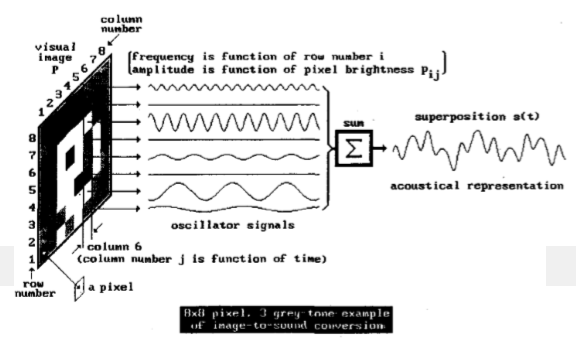
\includegraphics[width=1\textwidth]{image_to_sound}
\caption{\label{fig:image_to_sound}}
\end{figure}
  
The images have a resolution of 64 * 64 pixels with 16 gray-tones per pixels.  

The experiment showed promising functionality to convert images to sound but lacks a field study test on people with blindness. Moreover, the advantages and disadvantages of this system is yet to be proved. This questions the reliability of the system since there is no recordings of testing data presented in the article of the experiment. However theory supports the system's functionality.  \todo{talk about the math can be used in other projects and be build upon}

\subsection{The Sound of Photographic Image}\label{sec:soundarticle}
\todo{most focus on point relevant for the project. please rework}

A use of images for conversion into sound was performed and described in a paper by Atau Tanaka, who is the chair of digital media and director of culture lab at Newcastle University.

The paper describes two processing methods that both converts images into sound.

The first method utilises two image series. The method used to create the sound from the image uses a temporary mapping and additive synthesis on raw grayscale images, by scanning every pixel. A bright pixel produces high notes and a dark pixel produces a low note. \todo{Ref. paper Tanaka}

The second method was used for an interactive art installation. The interactive art consisted of a wooden structure with panels covered in rice paper to display Tanaka's pre-processed images from one of the image series. The images were processed through re-synthesis processes, where the frequency bands where quantisized to whole tones and pentatonic were mapped in which the key notes are played one at a time. The images were projected with negative pixel values creating a inverted image of the original and each row displayed different frequency ranging from low to high frequencies. An example of this result can be seen in the Figure below.  

(figure 5) \todo{ref to figure}

To capture human interaction, an infrared camera on top of the installation used viewers silhouettes as a layer on the negative image which was used to reveal the original black and white image for the viewer, as seen in Figure 6.

(figure 6) \{ref to figure}

This interaction also affected the produced sound which were based on the brightness of the processed image and thus produced new sounds. 

This visualisation of sound through images shows dynamic functionality of a interactive system, which utilises human interaction to alter a preprossed image. However, since there was no evaluation of this exhibit, it is difficult to know of the practical application of these methods. This is due to it being used in an artistic way, instead of a practical one.   
 

\section{Methods used to evaluate}\label{sub:methodsusedtoevaluate}






\section{State of the art}\label{sec:stateart}

\subsection{Sonic Photo}\label{sub:sonic}
\todo{make into reference}
Can be found here: http://www.skytopia.com/software/sonicphoto/

Sonic photo is a program that allows the user to transform an image into sound. The user can load an image into the program, and adjust various parameters to modify the resulting audio. The parameters include  frequency(Hz), brightness, tone, harmony quantization, etc.

\todo{more general information about the program. Which points to we want to make, by writing about this program?}
%!TEX root = ../master.tex
\chapter{User Needs in Context Study}\label{ch:userstudy}



%!TEX root = ../master.tex
\chapter{Final Problem Statement}\label{ch:finalproblem}



%!TEX root = ../master.tex
\chapter{Design}\label{ch:design}
\todo{This part needs rework. Write after chapter is done.}
This chapter will cover the design iterations and the decisions that were made. 

\section{Conceptual model}
This project will work with audiolisation of image. The initial design is focused on the conversion of images into an audio signal. Each pixel has an intensity value which can be converted into a range that fits the human hearing of 20 to 20.000Hz (insert refrence). The output of this operation can then be manipulated by audio processing filters (insert refrence).

The concept includes a control interface in the artefact. It allows the user to have control over the output in real time, as the control interface will change how the filter effect will modify the image-created audio. This gives the user agency of how the output will sound. To allow the user to create even more unique sounds, multiple filter can be applied simultaneously. This allows for a wide range of artistic expression, as the user will have control over the audio output.

\section{Peripheral devices}
The user has to be able to affect the audio that the image generates by interacting with a physical interface. The system will apply an affect which can be modified through a physical scalar which changes the variable range of the power of the effect from 0\% to 100\%, or in digits 0 to 1. For this interface these different variations of a physical scalar has been considered: 

\begin{itemize}
\item Button
\item Pressure sensor
\item Ultra sonic distance sensor
\item Potentiometer
\item Slider
\item Bend sensor
\end{itemize}

\begin{figure}[!h] 
\centering
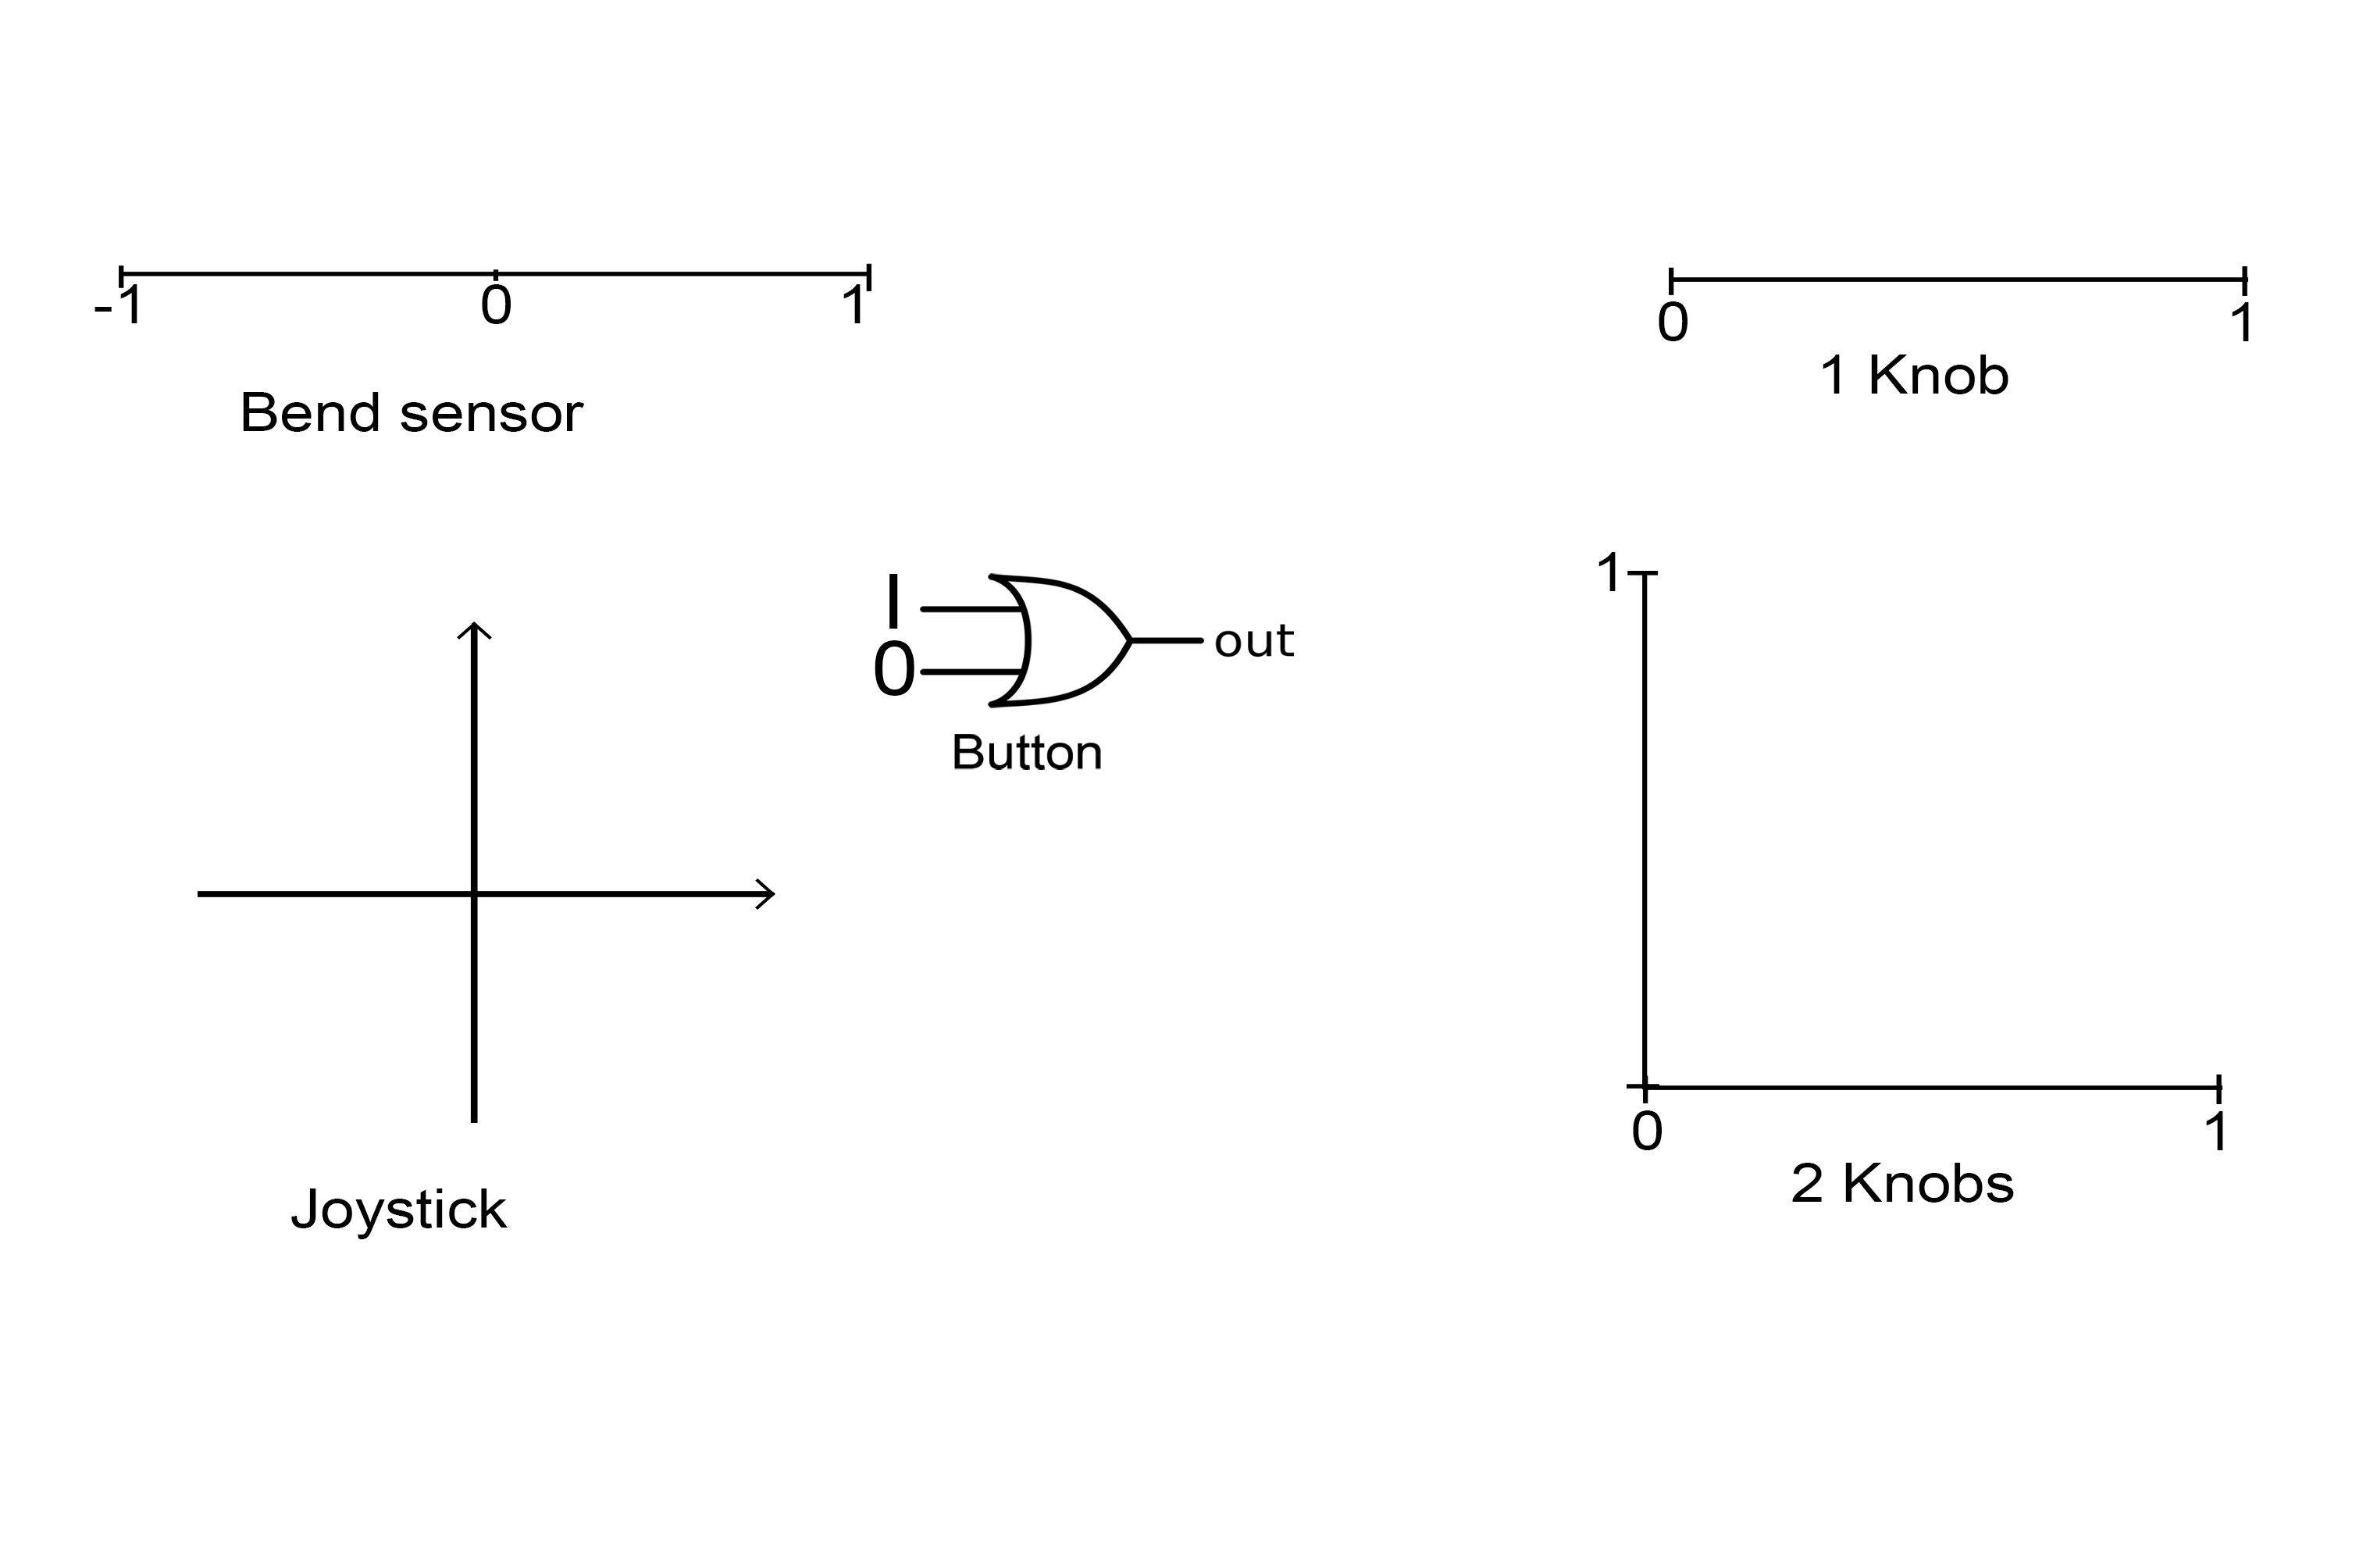
\includegraphics[width=1\textwidth]{Axis}
\caption{\label{fig:axis}}
\end{figure}


\todo{talk about what is the preference of different interfaces for the user (after test)}

Each of these peripheral devices makes the user interact with the prototype differently and changes the function of each device.

Figure \ref{fig:axis} shows the scales of which the different devices operate on, and how many different axis they are able to manipulate and to what length.
 
The joystick work by incorporating a variable on each axis, such that when the joystick is moved it alters the variables on the axis. 

There are multiple variable resistors to choose from. One of them being a knob the user can turn, which scales from 0 to 1 as well as a bend sensor that scales from negative 1 to positive 1. When the user alters the resistance in the system, the Arduino registers the change and send back a signal to the software in order to change the effect.

The way that these devices would be used, are as variable controller for the effect itself. Depending on what device is chosen, the integration for the user will be different. This will be tested in the iterations of the prototype and discussed further to make sure that the interface is user-friendly and easy to understand. 

\todo{expand upon the advantages and disadvantages of the different categories of devices}

\section{Early sketches and testing}
While sketching ideas for the design, the group encountered the obstacle of not knowing which electrical components to use. Therefore component test was with the purpose of deciding which component is the most intuitive to use. 

The test used the components mentioned in !insert ref til tidligere section! but there was two different buttons, a normal push button and a telegraph like button and three different potentiometers!fix this and describe which buttons there actually was!

These components were all mounted on a cardboard plate as seen on the figure below.

!!insert figure of pap thing og beskriv det!!

The test was conducted on 10 participants, all fellow students from Medialogy. The participants were explain by test facilitator 1 how each component worked and how to interact with them. They were told that they had to use all of the components one at a time in a numeral order and think out loud when using the components. Test facilitator 2 turned the volume of the music up and down, corresponding to how much the participant !!turned/clicked/slid/moved their hand!!.

Results showed that the participants preferred using the slider, showed on the figure below, when changing the volume of the music. New design sketches were created based on this result.

\section{Sketch ideas for interface}
Hej Knud. Se venligst bort fra dette afsnit
husk at forklare om feedforward og percieved affordance

\section{The chosen sketch}
Hej Knud. Se venligst bort fra dette afsnit
Forklar i details om sketchen, hvorfor vi valgte den og indsæt statediagrammet

\section{Interface low-fi test}
The chosen sketch was made into a paper mock-up to test the percieved affordance and the feedforward. Since it was a paper mock-up, no electronic components were used. What should have been the audio feedback was replaced with an drawing of a light bulb in order for understanding the intention of changing the intensity of an object. 

The mock-up was tested on 6 fellow Medoialogy students. Test facilitator 1 explained how the interface worked and asked the participant to execute the following tasks:
\begin{itemize}
\item Turn on the device
\item Turn on slider 1
\item Change the intensity of the illumination of light bulb 1
\item Turn on slider 2
\item Change the intensity of the illumination of light bulb 2
\item Turn on both sliders
\item Change the intensity of both or individually both light bulbs
\item Turn off the device
\end{itemize}





%!TEX root = ../master.tex
\chapter{Implementation}\label{ch:implementation}

\section{Tools used}\label{sec:toolsused}
!Anna rettelse. Tjek om ok eller ej!
The tools used in this project is an Arduino and the software Pure Data. 
An Arduino is a micro controller that allows the user to code and create their own circuits using various components. The Arudino is responsible for the control of the physical interface which the user has available.
Pure data is a C/C++ based coding language which utilises pre-constructed blocks of code which have to be connected to one another. Pure data is the code implemented in the project which is responsible for the audio and image processing. The image processing is conducted by utilising a library called Gem. 
A library called Firmata allows the Arduino to communicate with the software on the laptop.


!Before!
The tools used in this project is Pure data and Arduino. 
Pure data is a C/C++ based coding language which utilises pre-constructed blocks of code which have to be connected to one another. Pure data is the code implemented in our project which is responsible for the audio and image processing. Gem is used for the image processing purpose, which is a library in Pura data that allows for various image processing and animation methods.  
Furthermore three different filters have been constructed and implemented using pure data.

An Arduino is a micro controller that allows the user to code and create their own circuits using various components, this allows for a wide range of purposes. In this project the Arudino is responsible for the physical interface which the user has available. 

\subsection{Audio filters}
In the domain of audio effects, the term "filters" describes effects that modify the partial amplitudes of audio signals according to their frequencies \cite{zolzer2011dafx}. Filters combine their input signal with delayed and modified versions of themselves and then filters out certain frequencies. If a delayed version of the input signal is added to the signal, it is called a feedfoward filter, and if the signal is added to a delayed version of itself, it is called a feedback filter. This makes feedback filters more tricky to work with, since their effects can essentially amplify themselves \cite{steiglitz1997digital}. In this case the amplification can continue forever, no matter if you feed the filter a new input signal or not. This continuous amplification is called an unstable filter. Inversely, a stable filter is one, where the response fades over time, tending towards zero. This way, you make sure that the response of the input signal will end, depending on how fast the response signal fades.

\begin{figure}
\centering
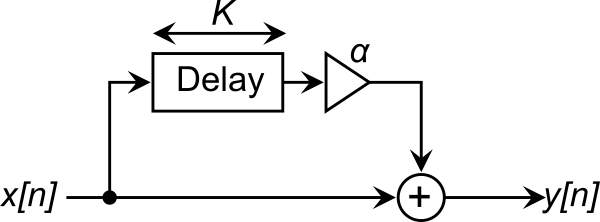
\includegraphics[width=0.5\textwidth]{feedforward}
\caption{Structure of basic feedforward filter.}
\label{fig:feedforward}
\end{figure}

\begin{figure}
\centering
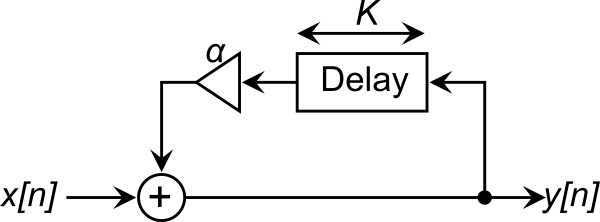
\includegraphics[width=0.5\textwidth]{feedback}
\caption{Structure of basic feedback filter.}
\label{fig:feedback}
\end{figure}

Filters can be put into three basic categories:
\begin{itemize}
\item \textbf{Pass filters} which lets defined frequencies pass, and reject the remaining. Examples of this type of filter are low-pass, bandpass and comb filters.
\item \textbf{Reject Filters} which is the inverse of a Pass filter. With this, defined frequencies are rejected and lets the remaining frequencies pass. Bandreject filters, also known as notch filters, are an example of this.
\item \textbf{Equaliser filters} which changes the amplitude of defined frequencies. This amplitude change can either be positive or negative, depending on the specific implementation of the filter. 
\end{itemize}

The filters used in the project is a bandpass, comb and high-shelf.

The comb filter used is a simple feedback filter, of the structure seen in Figure \ref{fig:feedback}. The summation of the delays creates constructive and destructive interference on the signal. This interference is at regular intervals, which gives the curve of the frequency response its distinct appearance, as seen in Figure \ref{fig:comb}. It is used to give an echo-like effect unto the input signal.

\begin{figure}
\centering
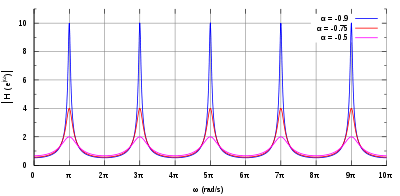
\includegraphics[width=0.5\textwidth]{comb}
\caption{Frequency response curve of comb filter.}
\label{fig:comb}
\end{figure}

The two other filters used are structured as biquads. \todo{CONTINUE FROM HERE}

The bandpass filter works by letting certain frequencies pass through, while rejecting all other frequencies. The accepted frequencies are defined by having a band with width \(B\) and a frequency \(f_0\) as its  centre point. This structure can be seen in Figure \ref{fig:bandpass}. The outermost points of the band \(f_L\) and \(f_H\) define the lowest and highest frequencies that are passed through, respectively. All frequencies lower than \(f_L\) and higher than \(f_H\) are rejected.

\begin{figure}
\centering
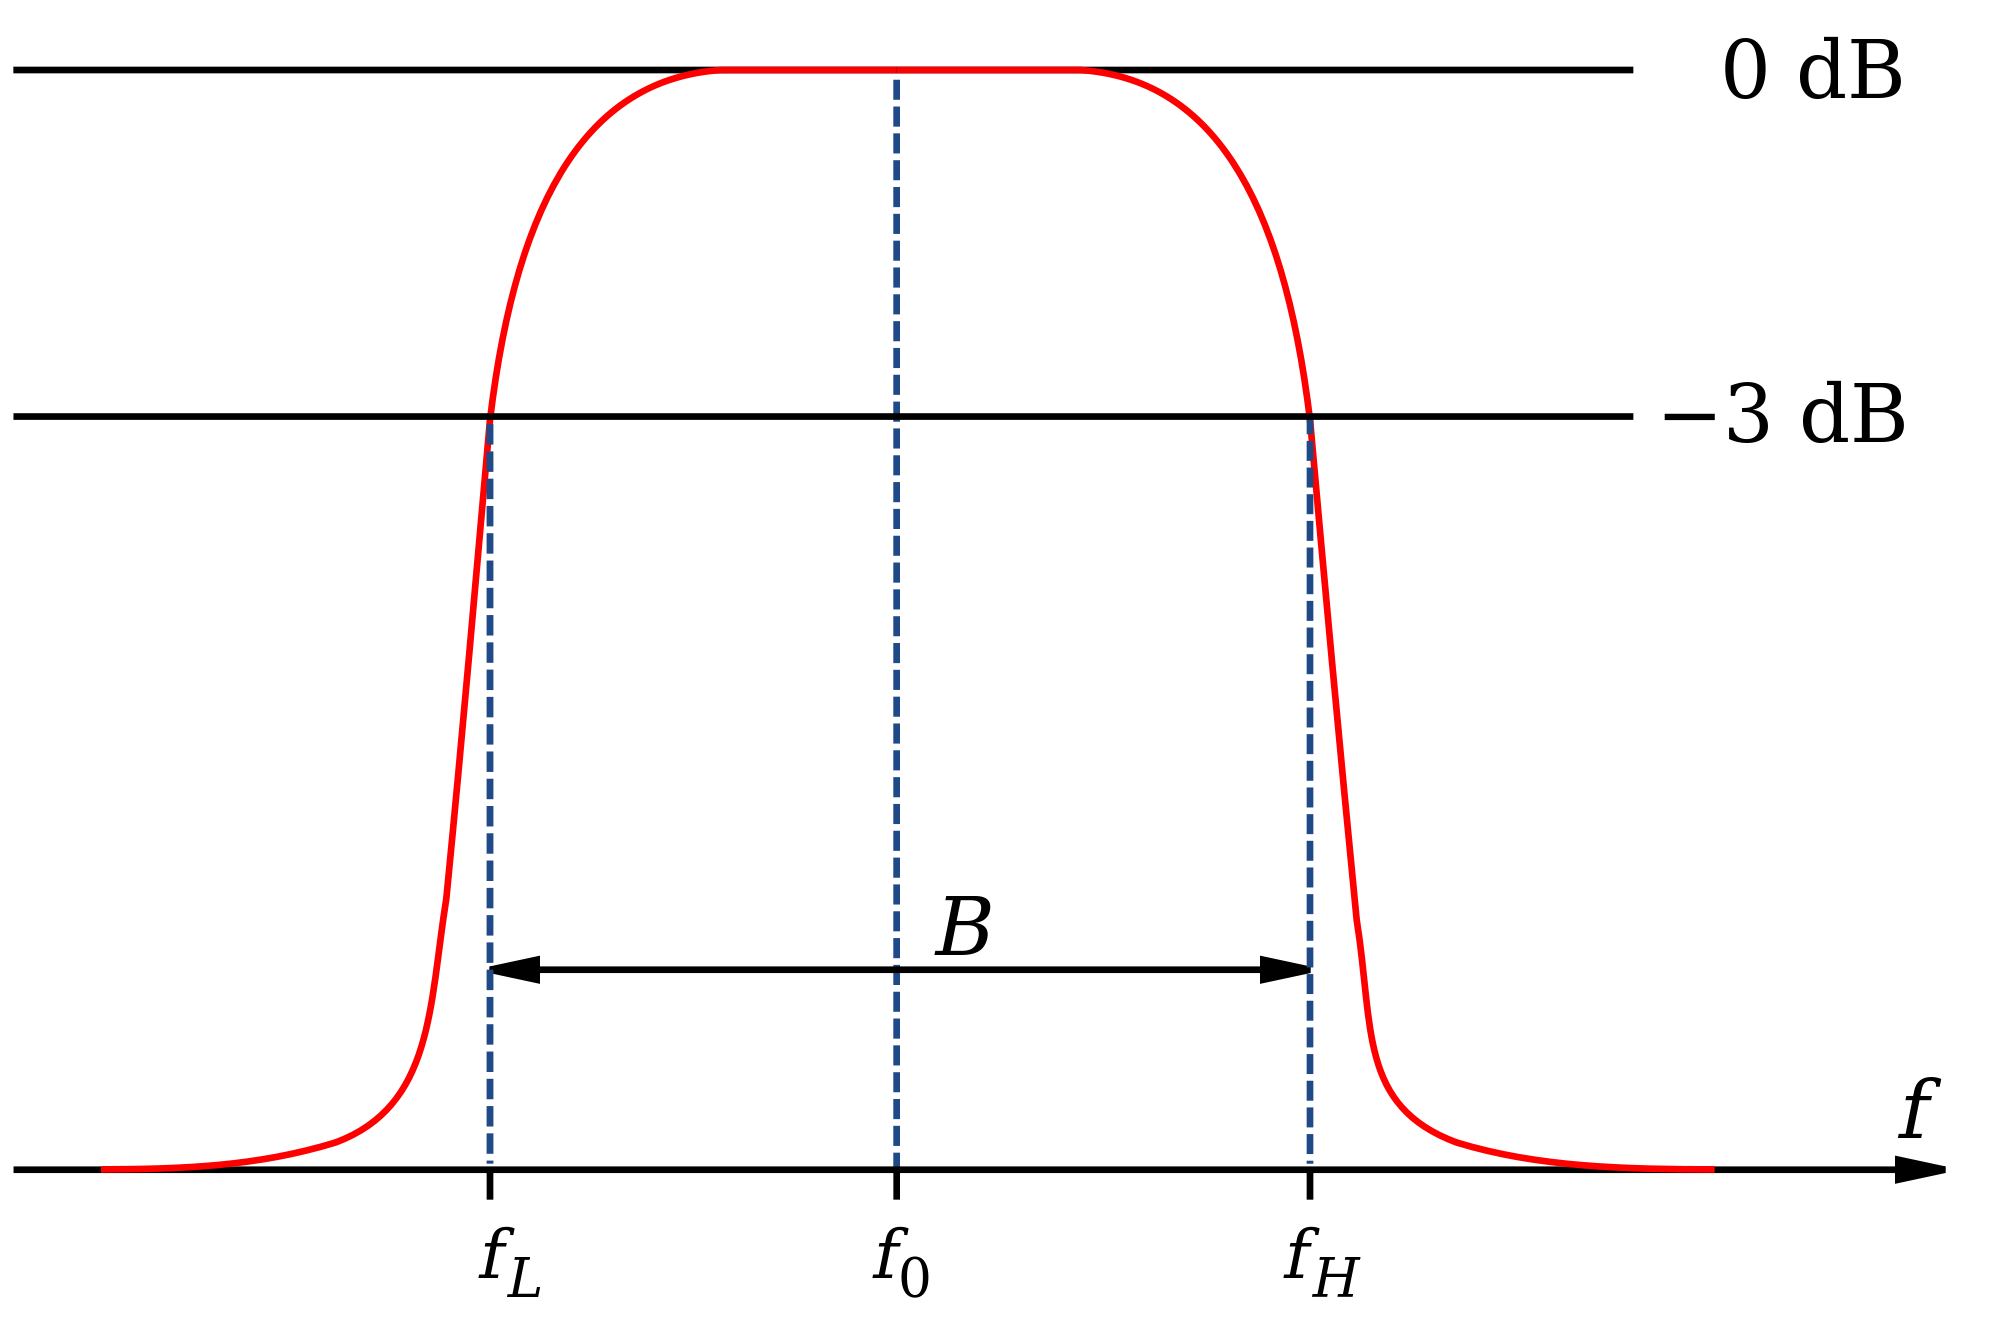
\includegraphics[width=0.5\textwidth]{bandpass}
\caption{Frequency response curve of bandpass filter.}
\label{fig:bandpass}
\end{figure}

\section{Software tools}\label{sec:softwareTools}
	\subsection{Image processing}\label{sub:imageprocessing}
	As the project revolves around pictures being audiolised, various image processing methods have been implemented. To get an image loaded into Pure data the library gem have been imported and applied. In gem it is possible to go through each pixel getting its RGB value as three different values. This is done using a double nested for-loop that is constructed using the expr function in Pure data, which allows for construction of consecutive if-statements. The first if-statement gives an output that is increased by 0.001 for every cycle if the input value is less than one. The second if-statement checks if the input value is greater or equal to one, if that is the case it adds 0.01 to a value starting at zero, which is then outputted. The last if-statement checks if the second input is greater or equal to 1, if that is the case subtract 1 from the value of the second input.
	
	Pipe is an object that delay the input given to it by a specific amount of milliseconds. It is used here to make sure that the program does not give a stack overflow error, and that it doesn't process the pixels too fast. By default in the program the pipe is set to 50 milliseconds since this allows the program to smoothly go through each pixel one by one. 
	When the pixel data is being processed in the program, it outputs the value of the three colour channels in the specific pixel, meaning that the output consists of three different value representing the R, G and B value. With the three RGB values it is possible to plot the values giving a graph of how the colour distribution is in the picture, but it is also possible to normalize the values into a signal by normalizing them from zero to one into negative one to positive one. By doing this the values have now been turned into a signal, which in terms should be able to produce a sound.

	\subsection{Audiolisation of image}\label{sub:audiolisationofimage} 
	Audiolisation of an image means to turn the image into some kind of audio, which is what the program explained in \ref{sub:imageprocessing} is programmed to do. 
	
	\subsection{Arduino}\label{sub:arduino}
	Arduino is a micro controller with open source software, that allows for custom coding in processing. Arduino has the capability to be connected to a breadboard for greater utility as the breadboard allows multiple components to be connected to a single Ardunio port, making it possible to create a 5 volt circuit using only a single pin. It is also possible to create a circuit using more than one pin, giving access to greater utility as each pin can be programmed separately in the program, giving each of the pins a unique functionality or making them become a duplicate, this would allow each pin to run a different circuit.
	Arduino is used in the project as the main control unit, as it is connects the physical interface to pure data. 
	
\section{Physical interface}\label{sec:physicalinterface}

	
	\subsection{Circuit diagram}\label{sub:circuitdiagram}
\begin{figure}
\centering
\includegraphics[width=0.5\textwidth]{circuit}
\caption{The circuit diagram.}
\label{fig:circuit}
\end{figure}

\begin{figure}
\centering
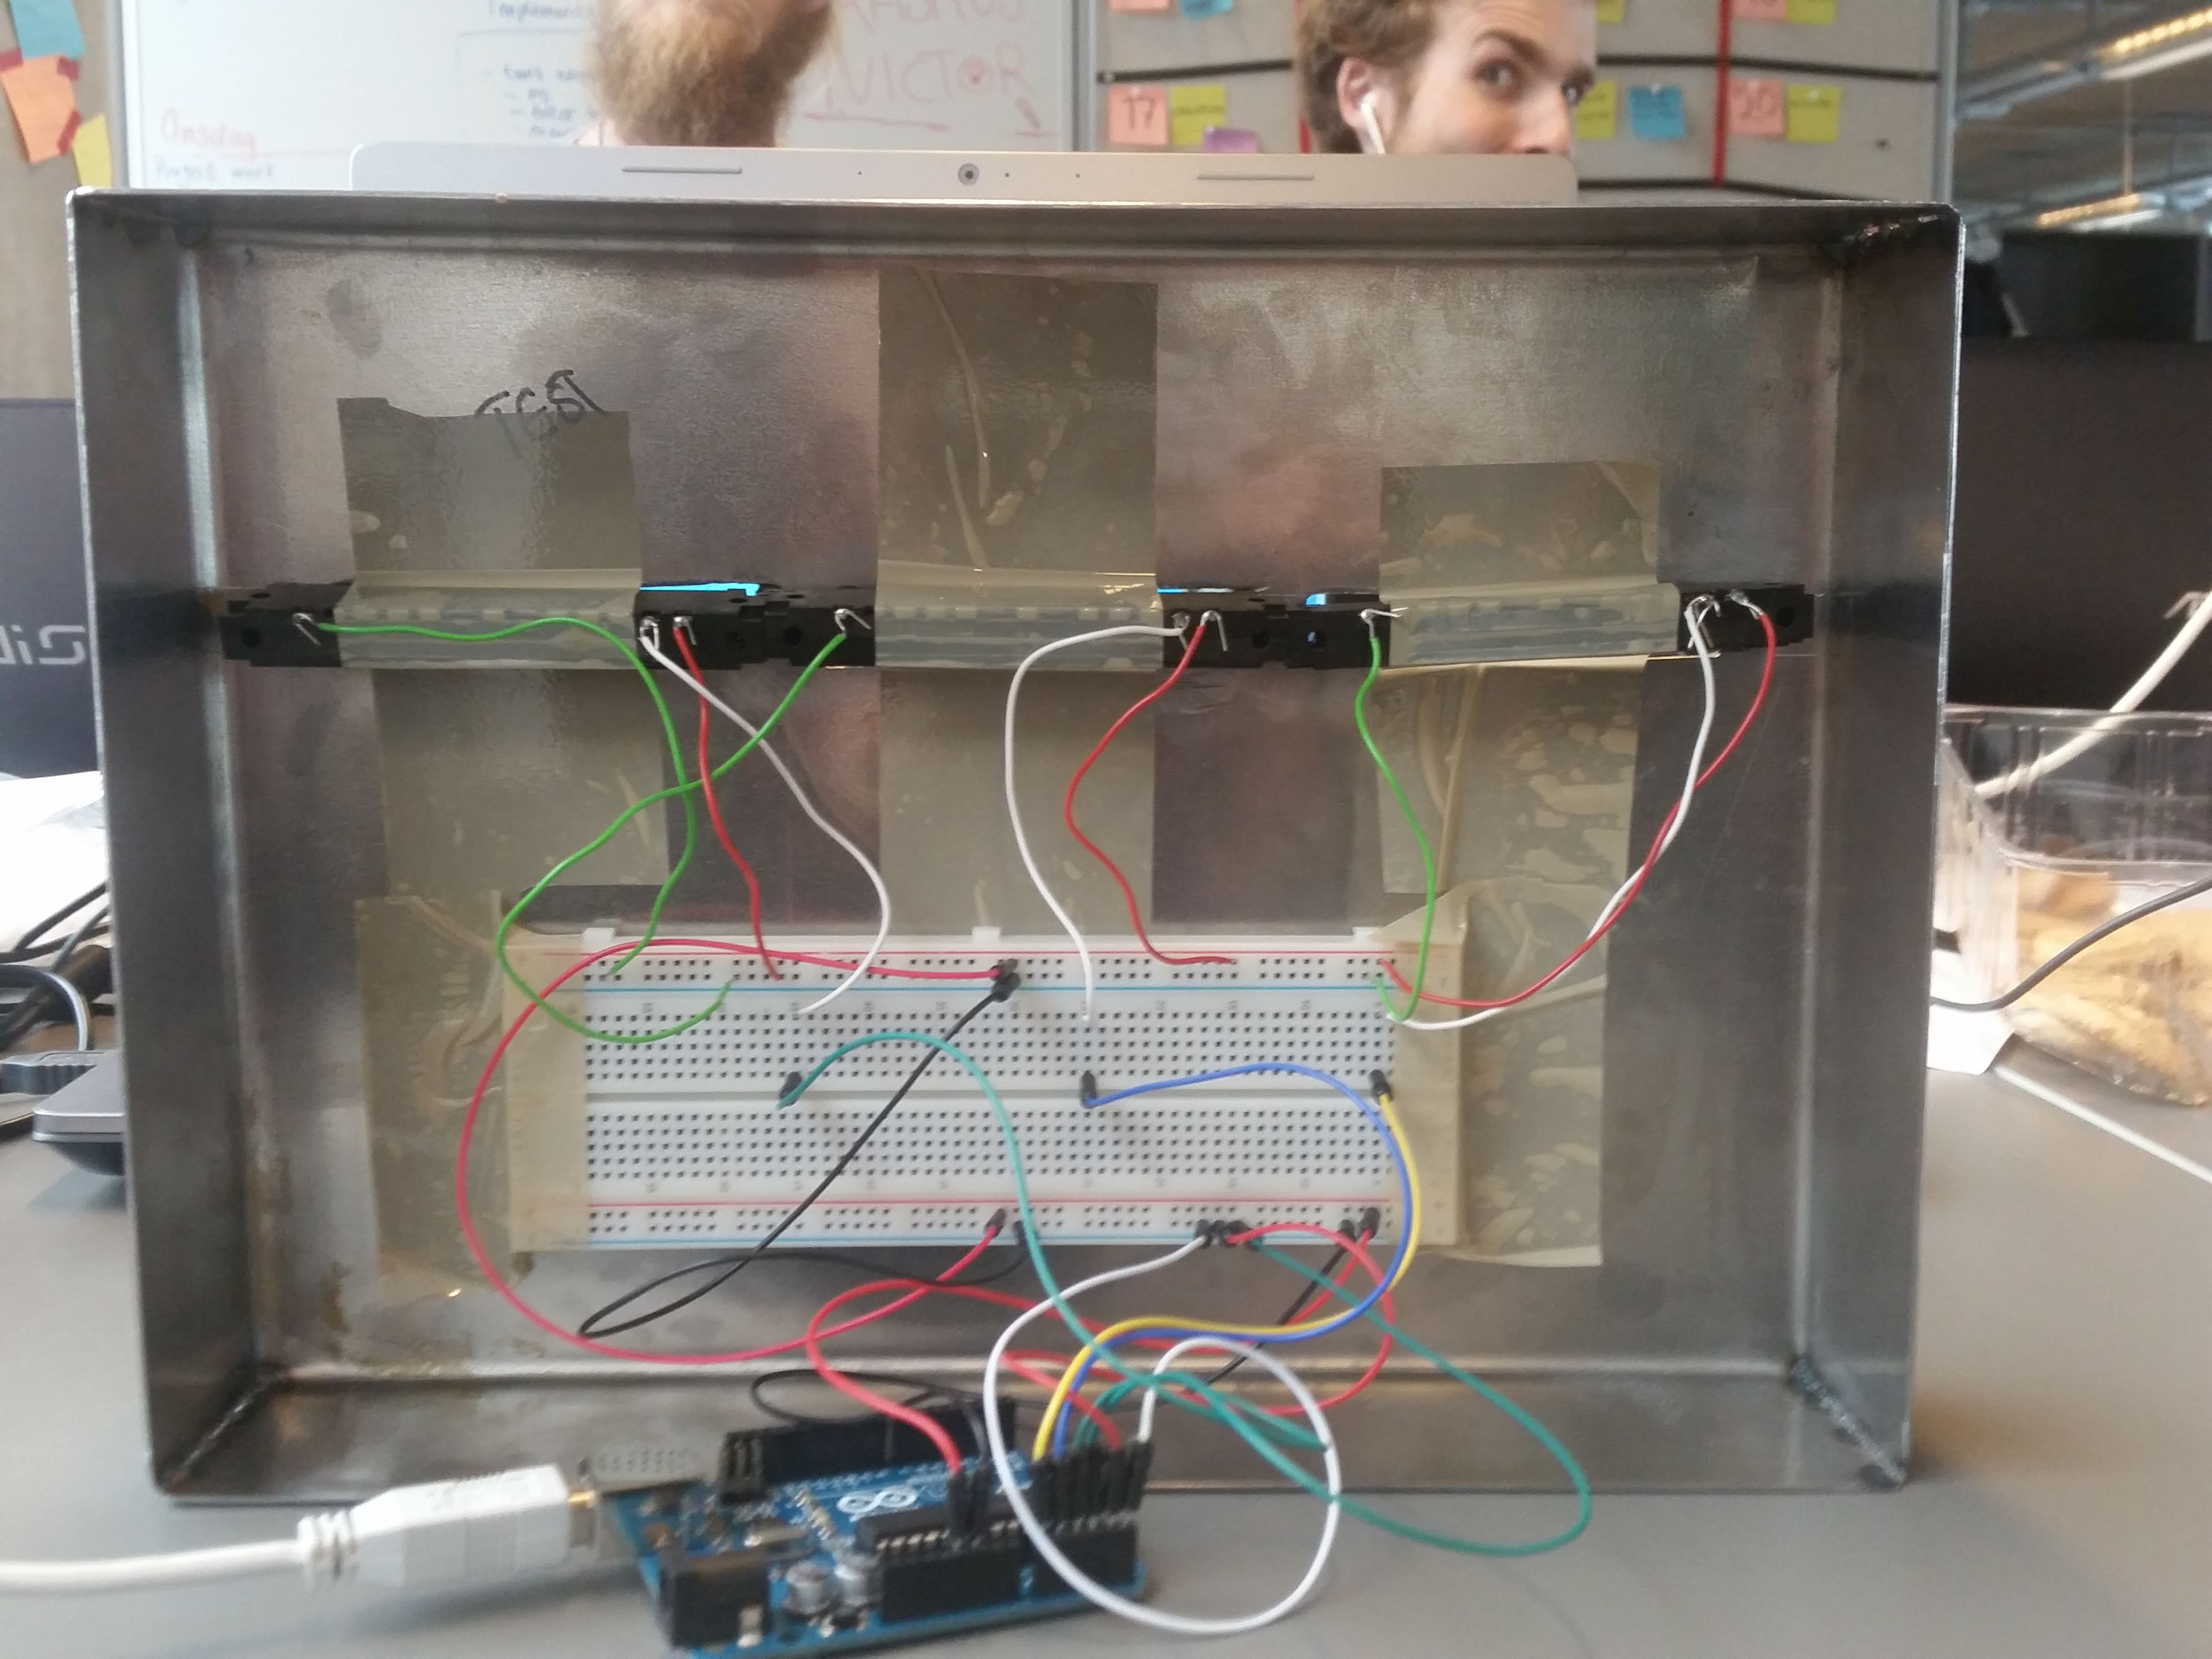
\includegraphics[width=0.5\textwidth]{backsideBox}
\caption{The circuit inside the box.}
\label{fig:backsideBox}
\end{figure}

\begin{figure}
\centering
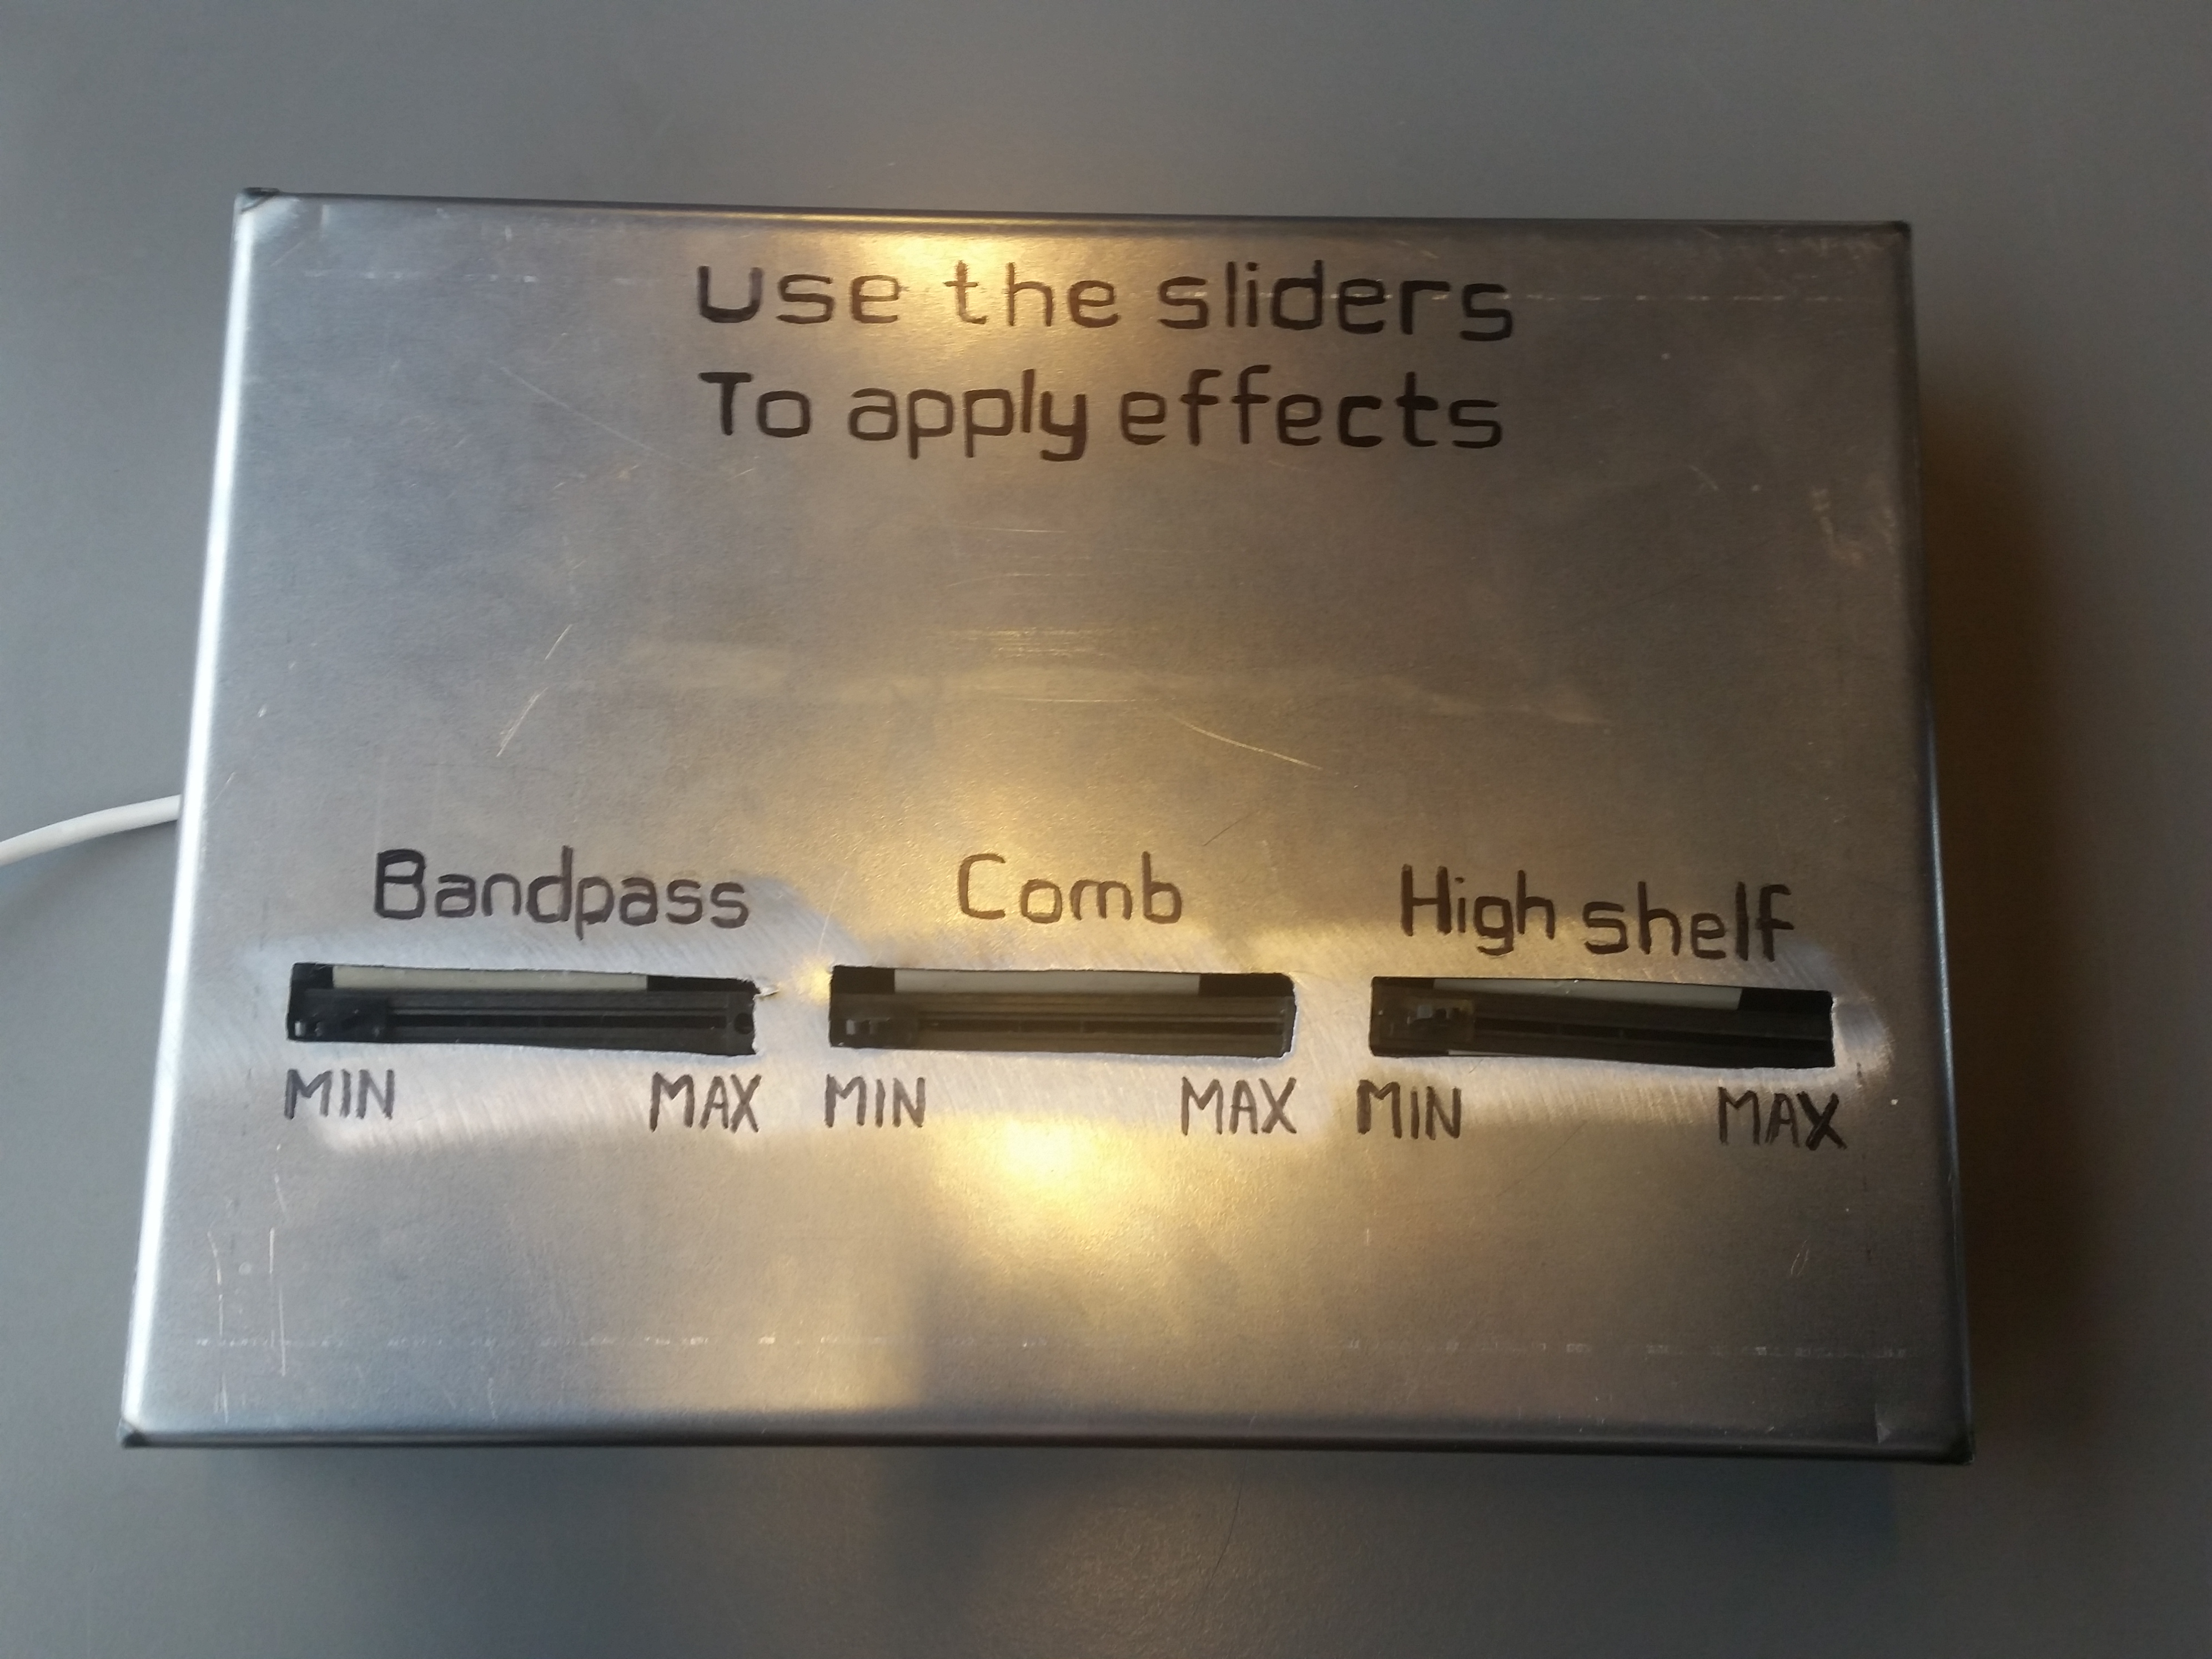
\includegraphics[width=0.5\textwidth]{frontBox}
\caption{The box containing the electronics.}
\label{fig:frontBox}
\end{figure}

	
	The interface works by utilising an Arduinos 5 Volt power supply and 3 slide potentiometer, placed in the lower half of the box, which send their output into the Arduino analogue ports, which is then interpreted by the code, which will be elaborated upon in Chapter \ref{ch:codeoverview} 

%!TEX root = ../master.tex
\chapter{Code Overview}\label{ch:codeoverview}
This chapter provides a detailed description of the software code. Figure~\ref{fig:flowchart} provides a simplified overview of the software.

\begin{figure}
\centering
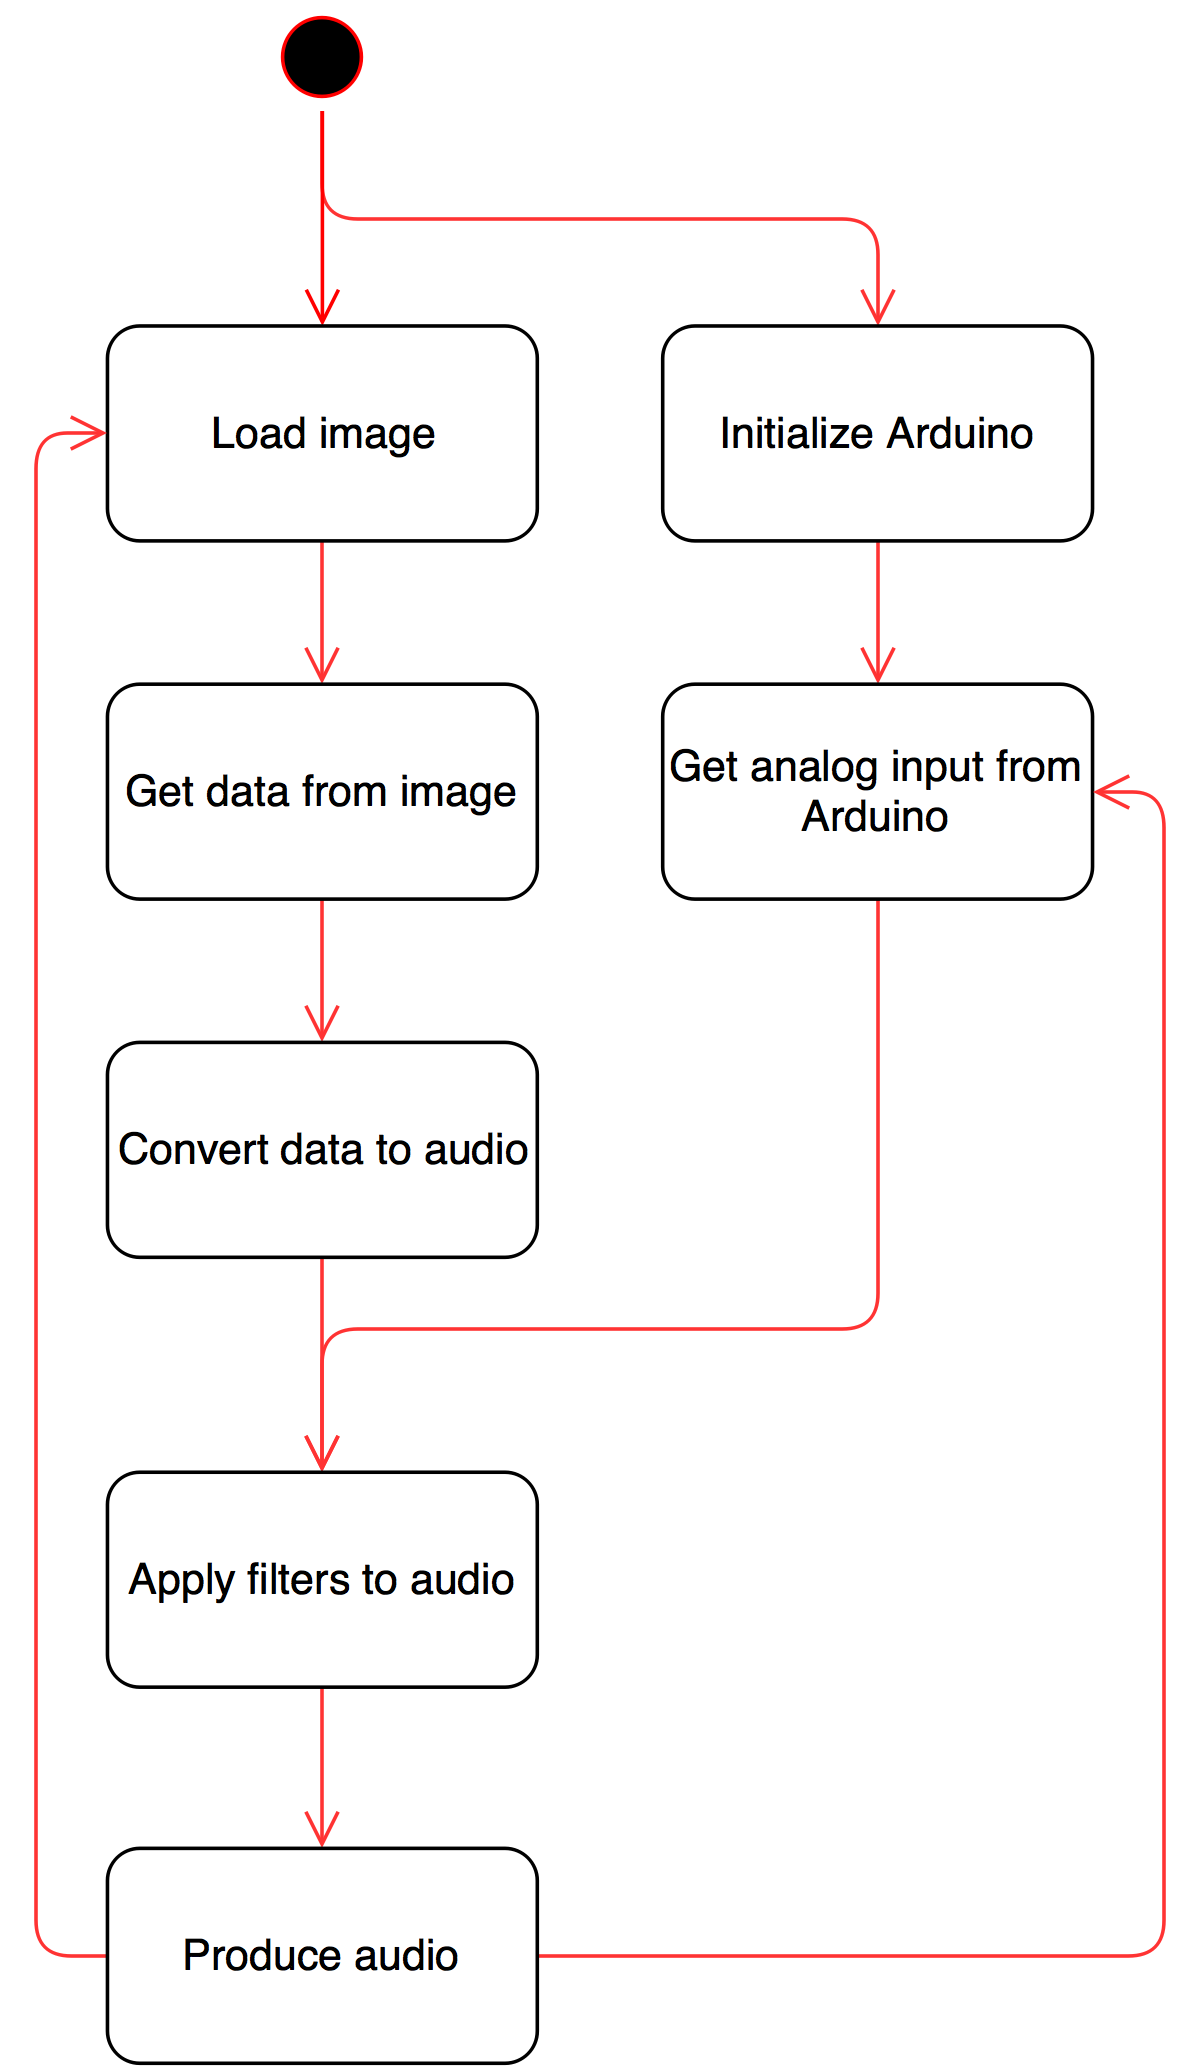
\includegraphics[width=0.5\textwidth]{flowchart}
\caption{Activity diagram showcasing the overall software.}
\label{fig:flowchart}
\end{figure}

\begin{figure}
\centering
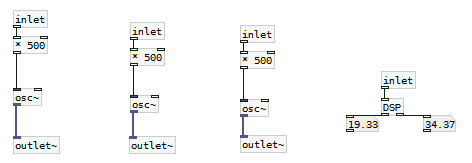
\includegraphics[width=1\textwidth]{Output}
\caption{The contents of \texttt{pd output}.}
\label{Fig:Output}
\end{figure}

\section{Audiolisation code}
When importing pictures into Pure Data a message called \texttt{open} is used. It takes a picture from a specific location and outputs it to \texttt{pix\_image} which prepares an image for further use. \texttt{pix\_image} sends the image into the \texttt{pix\_draw} which draws the image directly onto the screen. After the images is drawn, it is then sent into the \texttt{pd imageprocessing} patch which can be seen in Figure \ref{Fig:Imageprocessing}. A simplified diagram of this patch can be seen in Figure~\ref{fig:ipflowchart}.

\begin{figure}
\centering
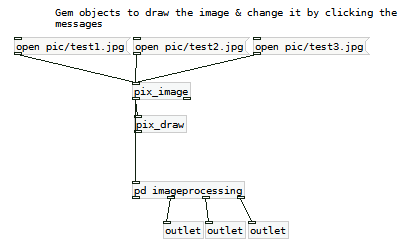
\includegraphics[width=1\textwidth]{Pdpictures}
\caption{The blocks that are responsible for image processing.}
\label{Fig:pdpicture}
\end{figure}

\begin{figure}
\centering
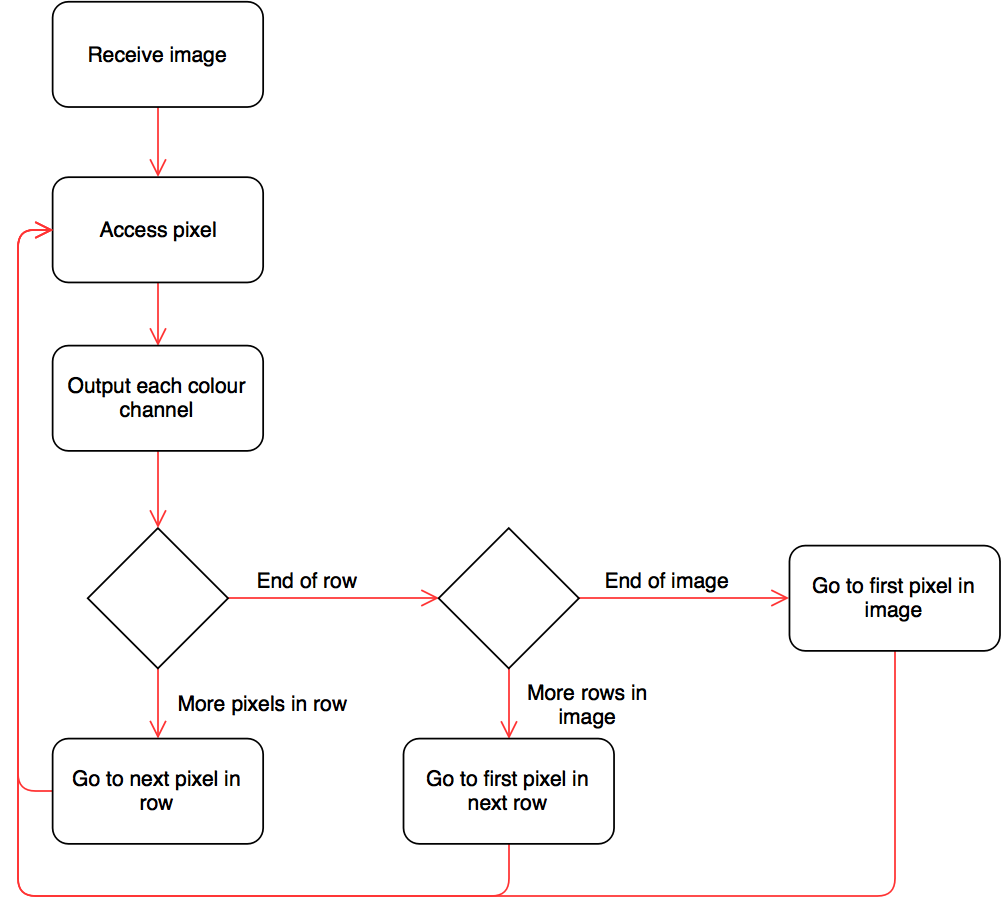
\includegraphics[width=0.5\textwidth]{diagram-ip}
\caption{Activity diagram of the image processing module.}
\label{fig:ipflowchart}
\end{figure}

A nested for-loop is implemented using an \texttt{expr} function. The for-loop is created using three if-statements, and taking advantage of the dataflow nature of Pure Data. It examines each pixel in the input image according to their x- and y-coordinate.
The loop goes from zero to one with an interval of 0.001. A \texttt{pipe} object is used to delay each iteration of the loop by 15 ms. When it reaches one it adds 0.01 to the variable \$f2 and resets \$f1 to zero to start over. When \$f2 hits one it resets to zero and the whole process starts over. The delay is used to ensure that the program does not cause a stack overflow. 
As the if-statements process the data, a set of sliders have been placed to visualise the current pixel position. These sliders move in real time as the image is processed. The information contained in the pixel at current position is outputted to the \texttt{pix\_data} object. It takes a pixel position and the image from \texttt{pix\_image} and outputs the values of the RGB channels into three different numbers boxes which are then outputted out of the \texttt{pd imageprocessing} patch. The output of the \texttt{pd imageprocessing} patch is inputted into the \texttt{pd output} patch. It takes the RGB values and converts it into a cosine wave frequency by multiplying the RGB value by 500 to make sure the frequency is within the range of human hearing. It sends the output to the three different filters; bandpass, comb and high-shelf which are explained in Subsection \ref{sub:audiofilters}. The output of the filters bandpass and high-shelf are coefficients, which are used by the biquad to create the filter effect. All three filter outputs are added together and sent to the \texttt{dac\~} object which outputs the audio to the speakers. 

\begin{figure}
\centering
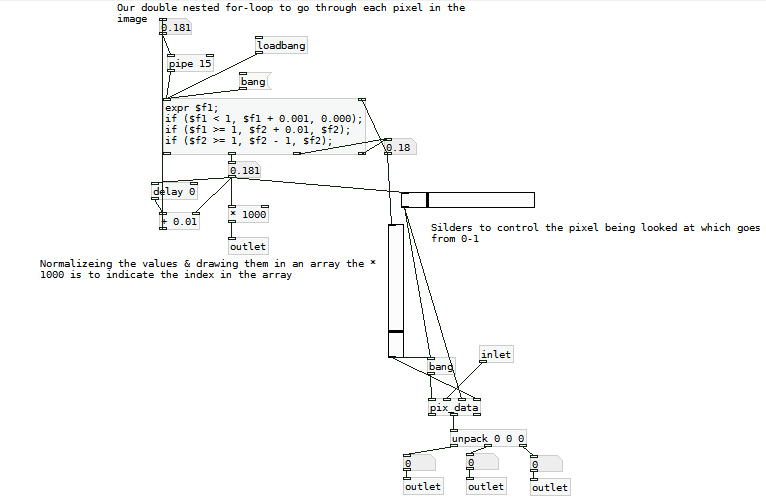
\includegraphics[width=1\textwidth]{Imageprocessing}
\caption{The contents of \texttt{pd imageprocessing}.}
\label{Fig:Imageprocessing}
\end{figure}


\section{Arduino code}
For the Arduino a \texttt{pd arduino} patch has been created, which can be seen in Figure~\ref{Fig:Inside_arduino}, which contains all the objects for the Arduino part of the code. It takes a number and a list of five numbers as inputs. The first single number defines which of the computer's serial ports will be used to access the Arduino. The list of numbers defines which analogue inlets are open and which are closed. Each analog inlet is associated with a position in the list, and the number determines whether a given inlet is active; '1' for active and '0' for inactive. This information is sent to the \texttt{pduino/arduino} object.

\begin{figure}
\centering
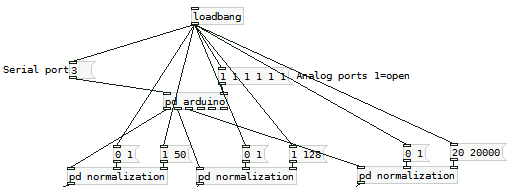
\includegraphics[width=1\textwidth]{Arduino_normalization}
\caption{The Arduino blocks for inputs and outputs.}
\label{Fig:Arudino_normalization}
\end{figure}

The \texttt{pduino/arduino} object sends all of its data into its single outlet. This data contains information from all active in/outlets, digital or analog, as well as information about the Arduino device and how it is performing. The only piece of information the software needs is the data from the analog inlet. The \texttt{route} object is used to filter out all data that does not contain the 'analog' label. Another \texttt{route} object is then used to sort the data according to the inlet it originates from. Finally a conversion is made so that the state of each inlet is represented with a floating point number between zero and one. This number changes when the user operates the slide potentiometer.


\begin{figure}
\centering
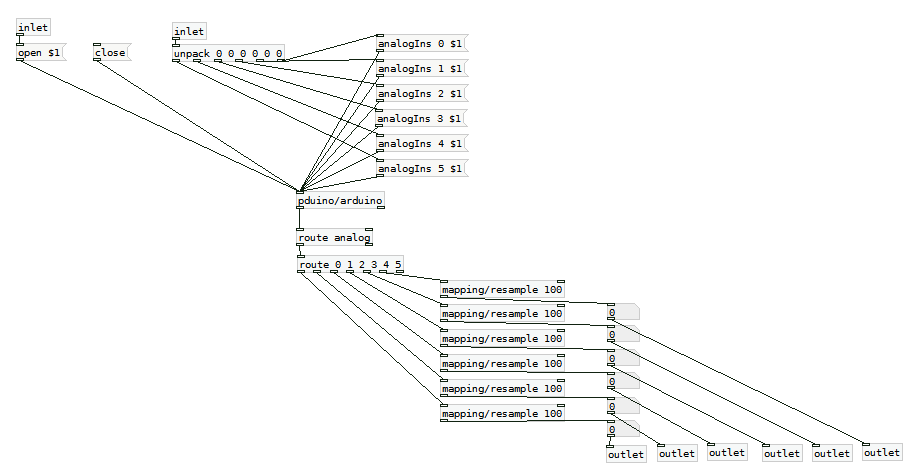
\includegraphics[width=1\textwidth]{Inside_arduino}
\caption{The contents of \texttt{pd arduino}.}
\label{Fig:Inside_arduino}
\end{figure}

The user defined parameters for the filters need coefficients in various ranges. To achieve this, a patch called \texttt{pd normalization} (see Figure \ref{Fig:Normalize}) is used to normalize the numbers from the analog inlets on the Arduino from a range of zero to one to a different range, depending on the filter. \texttt{pd normalization} has three inlets; one for the raw data, one for the original data range, and one for the desired range. The patch then applies the equation $\frac{max'-min'}{max-min}\cdot (data-max)+max'$ where max' and min' make up the desired range, and max and min make up the original range. The result is passed to the outlet which provides one of the filter coefficients for each filter. For the comb filter the delay is altered, for the high-shelf filter the gain is altered, and for the bandpass filter the center bandwidth is altered.

\begin{figure}
\centering
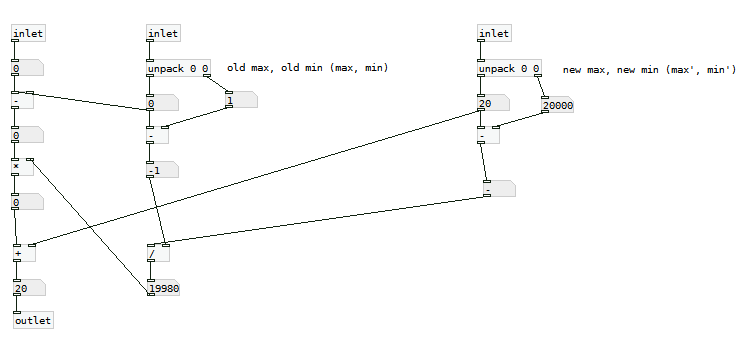
\includegraphics[width=1\textwidth]{Normalize}
\caption{The contents of \texttt{pd normalization}.}
\label{Fig:Normalize}
\end{figure}
%!TEX root = ../master.tex
\chapter{Final Prototype}\label{ch:finalprototype}


%!TEX root = ../master.tex
\chapter{Evaluation}\label{ch:evaluation}
This chapter will describe the evaluation process of the finished prototype. The chapter is spilt into three subsections: a planning section, actual evaluation description and analysis of evaluation results. 

\section{Further Context}\label{sec:furthercontext}
\todo{Explain additional functionality: draw on image to change the sound} 

\section{Planning of evaluation}
This section will describe the thoughts the project group made before the actual evaluation test were made. The section will show a description of the evaluation tasks and questions there were planned to be asked during the test. 

What do we want out of this test? / what are we testing for / 

\begin{itemize}
\item The user can alter the output by applying filters.
\item The user understands the interface  
\item The prototypes usability is over 80 percent of the users satisfaction.
\end{itemize}

Possible Interview questions
\begin{itemize}
\item What did you experience when manipulating with the sliders?
\item Where you confused about the design?
\item was the “text” helpfull to you?
\item Any other thoughts?
\end{itemize}

Assignments for the user to solve during the test 
\begin{itemize}
\item Turn on echo
\item Turn on echo and comb
\item Turn off comb
\item Turn on bandpass 
\end{itemize}


The test set up was planned to be held in a quiet area with one test participant at the time, located at Rendensburgade 14 (The Create building) it was planned to conduct the test on at least 12 people (2 test people pr. group member) 


Technical evaluation 


\section{Evaluation test}
This section will give a description of the set-up, procedure and results of the actual evaluation test of the final device. 

\begin{figure}[!h] 
\centering
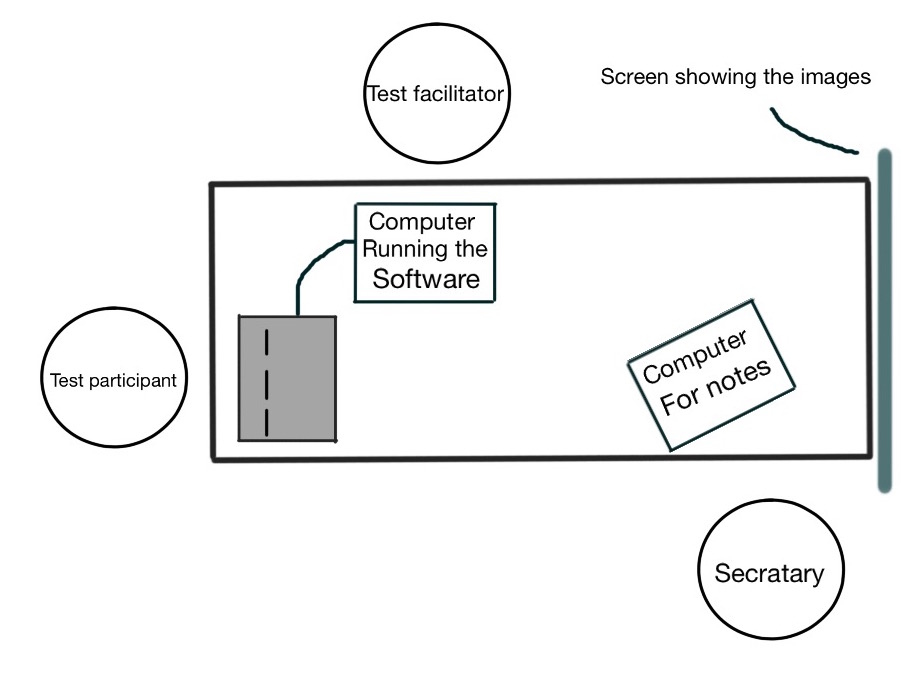
\includegraphics[width=1\textwidth]{testsetup}
\caption{\label{fig:testsetup} Illustration of the test set-up.}
\end{figure}

The final test was conducted on 15 test participants from Aalborg University in their 20's. The participants consisted of 14 students from medialogy and one student from Art \& Technology. \todo{dette kan bruges i diskution, da vi ville have faaet mere variation i resultaterne hvis vi fx. havde testet paa museumsgaester i alle aldre} The test took place in a small closed room located at Rendsburggade 14. The test was conducted by a test facilitator; who interviewed the participants and instructed which tasks to perform while observing the software during the test. During the testing a secretary would take notes of the entire test. Furthermore, the prototype was placed in front of the participants and a laptop was used to display the two pictures the project group decide to use during the test. The facilitator would change the picture on the laptop since it was not automatised and worked independently from the actual software and was only used to display the pictures.   

\begin{figure}[!h] 
\centering
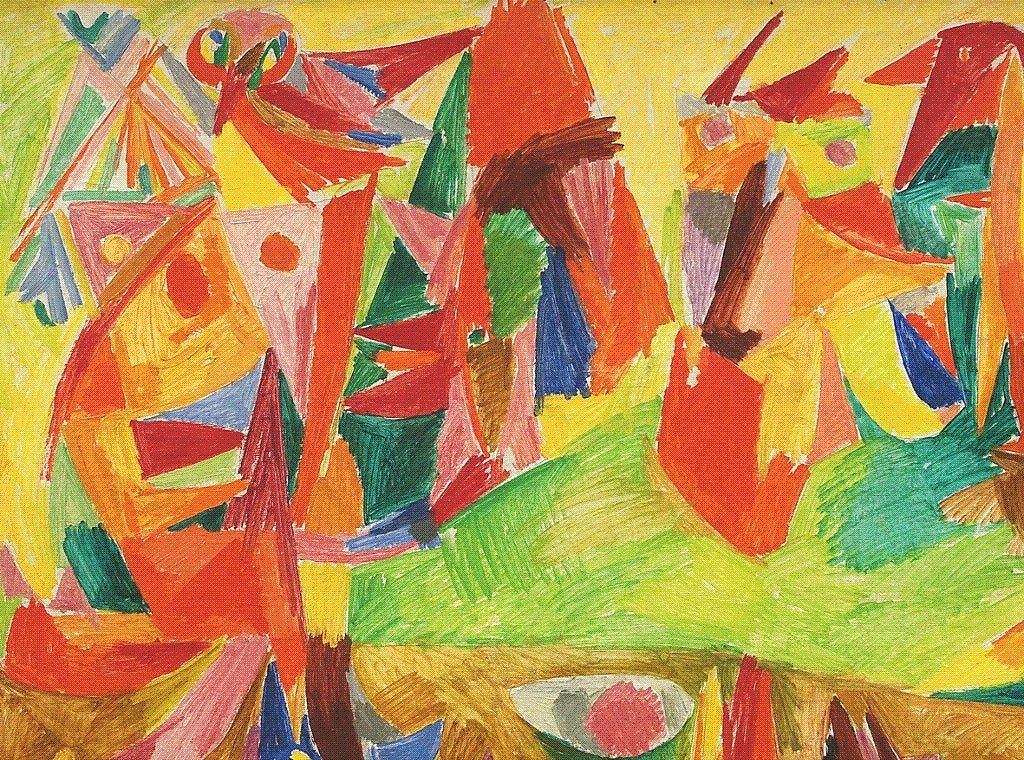
\includegraphics[width=1\textwidth]{asger}
\caption{\label{fig:asger} Asger Jorns "Trolden og Fuglene" 1944.}
\end{figure}

\begin{figure}[!h] 
\centering
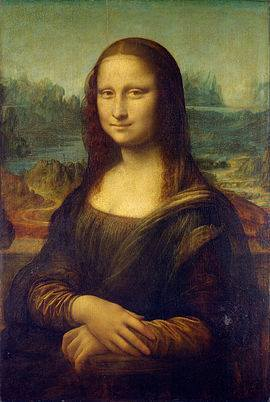
\includegraphics[width=0.5\textwidth]{monalisa}
\caption{\label{fig:monalisa} Leonardo Da Vinci "Mona Lisa" 1503-1517.}
\end{figure}

The test was carried out by welcoming the test participants in the room, one at the time. The participants were places at the end of the table and was asked to sign a consent form. The facilitator then started the test by introducing the overall project and explaining what the participant was expected to do during the test. The facilitator conducted the test by using the script shown below:


\section{Script}
The following text is the actual script, followed during the test.

Hello and thank you for wanting to participate in this test. We are group 30.

Our prototype takes an image and turns it into a sound. During this test we will give you a few different assignments and ask you questions during the test. This is a test of the product, and we prefer you to think out loud during the test.

//Mona Lisa is shown on the screen 
Questions: 


\begin{itemize}
\item What do you think you have to do with this product?
\item What happens when you manipulated with the sliders?
\item Can you hear a difference between “MIN” and “MAX”?
\item Can you hear a difference between the effects?
\item Is the “help text” helpfull to you?
\item Is the help text clear?
\item Any other thoughts?
\end{itemize}



/* Now we will change the images to Asgar Jorn */
\begin{itemize}
\item Do you hear the difference between the two pictures?
\item Why do you think there is a difference between the images?
\item Can you hear a difference between 'MIN' and 'MAX'?
\item Can you hear a difference between the effects?
\end{itemize}


Any other overall thoughts?

\section{Evaluation results}
Comb filter results

\begin{table}[!h]
\centering
\caption{}
\label{tab:comb}
\begin{tabular}{|l|c|c|c|c|c|c|c|c|c|c|c|c|c|c|c|c|c|}
\hline
\multicolumn{18}{|c|}{Can you hear the difference between the 'MIN' and 'MAX' on the Comb filter?} \\ \hline
\multicolumn{2}{|l|}{} & \multicolumn{15}{c|}{Amount of participants} & \textbf{Total} \\ \hline
\multirow{2}{*}{\begin{tabular}[c]{@{}l@{}}Mona \\ Lisa\end{tabular}} & Yes &  &  &  &  &  &  &  &  &  &  &  &  & X &  &  & \textbf{1} \\ \cline{2-18} 
 & No & X & X & X & X & X & X & X & X & X & X & X & X &  & X & X & \textbf{14} \\ \hline
\multirow{2}{*}{\begin{tabular}[c]{@{}l@{}}Asgar \\ Jorn\end{tabular}} & Yes &  &  &  &  &  &  &  &  &  &  & X &  & X &  &  & \textbf{2} \\ \cline{2-18} 
 & No & X & X & X & X & X & X & X & X & X & X &  & X &  & X & X & \textbf{13} \\ \hline
\end{tabular}
\end{table}

Bandpass Results
\begin{table}[]
\centering
\caption{}
\label{tab:bandpass}
\begin{tabular}{|l|c|c|c|c|c|c|c|c|c|c|c|c|c|c|c|c|c|}
\hline
\multicolumn{18}{|c|}{Can you hear the difference between the 'MIN' and 'MAX' on the Bandpass filter?} \\ \hline
\multicolumn{2}{|l|}{} & \multicolumn{15}{c|}{Amount of participants} & \textbf{Total} \\ \hline
\multirow{2}{*}{\begin{tabular}[c]{@{}l@{}}Mona \\ Lisa\end{tabular}} & Yes & X & X &  & X & X & X & X &  & X & X & X & X & X &  &  & \textbf{11} \\ \cline{2-18} 
 & No &  &  & X &  &  &  &  & X &  &  &  &  &  & X & X & \textbf{4} \\ \hline
\multirow{2}{*}{\begin{tabular}[c]{@{}l@{}}Asgar \\ Jorn\end{tabular}} & Yes & X & X & X & X & X & X & X &  & X & X & X & X & X &  & X & \textbf{13} \\ \cline{2-18} 
 & No &  &  &  &  &  &  &  & X &  &  &  &  &  & X &  & \textbf{2} \\ \hline
\end{tabular}
\end{table}


High shelf results
\begin{table}[]
\centering
\caption{}
\label{tab:highshelf}
\begin{tabular}{|l|c|c|c|c|c|c|c|c|c|c|c|c|c|c|c|c|c|}
\hline
\multicolumn{18}{|c|}{Can you hear the difference between the 'MIN' and 'MAX' on the High Shelf filter?} \\ \hline
\multicolumn{2}{|l|}{} & \multicolumn{15}{c|}{Amount of participants} & \textbf{Total} \\ \hline
\multirow{2}{*}{\begin{tabular}[c]{@{}l@{}}Mona \\ Lisa\end{tabular}} & Yes & X & X & X & X & X & X & X & X & X & X & X & X & X & X & X & \textbf{15} \\ \cline{2-18} 
 & No &  &  &  &  &  &  &  &  &  &  &  &  &  &  &  & \textbf{0} \\ \hline
\multirow{2}{*}{\begin{tabular}[c]{@{}l@{}}Asgar \\ Jorn\end{tabular}} & Yes & X & X & X & X & X & X & X & X & X & X & X & X & X & X & X & \textbf{15} \\ \cline{2-18} 
 & No &  &  &  &  &  &  &  &  &  &  &  &  &  &  &  & \textbf{0} \\ \hline
\end{tabular}
\end{table}

Is the "help text" useful you you?
\begin{table}[!h]
\centering
\caption{}
\label{tab:helptext}
\begin{tabular}{|l|c|c|c|c|c|c|c|c|c|c|c|c|c|c|c|c|}
\hline
\multicolumn{17}{|c|}{Is the "help text" usefull to you?} \\ \hline
 & \multicolumn{15}{c|}{Amount of participants} & \textbf{Total} \\ \hline
Yes &  & X & X & X & X & X & X & X & X & X & X & X & X & X & X & \textbf{14} \\ \hline
No & X &  &  &  &  &  &  &  &  &  &  &  &  &  &  & \textbf{1} \\ \hline
\end{tabular}
\end{table}

Can you hear a difference between the two images?
\begin{table}[!h]
\centering
\caption{}
\label{tab:twoimagedifference}
\begin{tabular}{|l|c|c|c|c|c|c|c|c|c|c|c|c|c|c|c|c|}
\hline
\multicolumn{17}{|c|}{Can you hear a difference between the two images?} \\ \hline
 & \multicolumn{15}{c|}{Amount of participants} & \textbf{Total} \\ \hline
Yes & X & X & X & X & X & X & X & X & X & X & X & X & X & X & X & \textbf{15} \\ \hline
No &  &  &  &  &  &  &  &  &  &  &  &  &  &  &  & \textbf{0} \\ \hline
\end{tabular}
\end{table}


\section{Results analysis}
This section describes the results found in the final test. The results were found by making a semi-structured interview and getting qualitative feedback by communicating directly with the user, using the script shown above. 

From the testing, 13 of the participants found it difficult to hear the difference between 'MIN' and 'MAX' when manipulating with the comb filter on both Mona Lisa and Asger Jorns picture. However, when using the Bandpass and High shelf, the user could hear a clear difference between the two filters when changing the values using the sliders. Two of the test participants had no clear comments regarding the difference between any of the filters. These answers was marked as "not clear for use" in case the test facilitator and secretary had misunderstood the participant's answer. 

Nine of the participants did not know the terms of the different filters, but they could distinguish a change in the output when manipulating with the sliders. Therefore, they did not know exactly what to listen for when manipulating with the sliders. Six of the participants from Medialogy knew the terms of the three filters. Even though six of the participants knew the terms of the filters, only two knew exactly what the filters did, and what they had to listen for when manipulating with the sliders. 

The interface was clear for all the participants and they knew how to use it, either by looking at the help text or at the sliders. None of the test participants had any trouble manipulating with the sliders. 

All of the participants could hear a clear difference between the colourful Asger Jorn painting and the darker Mona Lisa painting. They all suspected the difference in the colours for being the reason for the difference in the sound. 

To sum up the overall thoughts on the product, the test participants found the device to be very easy to use, even though most of them did not know what the filters actually did or what the names of the filters meant. 

\todo {One particpant was asking if the later iteration would show the context between the picture and sound to find a balanced and satisfying output}. 
%!TEX root = ../master.tex
\chapter{Discussion}\label{ch:discussion}
This chapter contains discussion of the entire project 

\section{Sources of error}

\todo{ ved ikke hvor jeg skal skrive det her, men det kommer lige her, skal sættes ind det rette sted og rettes i}
 Since the final test were only conducted on 14 medialogy students and one Art \& technology student, is it hard to say if our product would be just as "easy to understand" for a normal museum visitor or any other user. To investigate if the product would be accepted among people with no knowledge of audio processing or people who are having trouble understanding "techical stuff I don't know" the optimal solution would be to test the product in context, in this case it could be at an art museum, where the test would be conducted on guests of the museum which could be people of all age groups. 
 
 \section{Contex of use}
 - During this project, two of the members of the project group visited the art museum Kunsten in Aalborg. The goal was to find out how the artefact could be used in context at the museum. 
 
 - how would the setup be so the visitors could draw a connection between the painting and the artefact 
 
 - pictures from Kunsten 
 
 - Results from the visit
 
 - show sketch of grandma at the art museum / solution. 
 
 - One of the test participants was unsure of the connection of the artefact and the paintings shown during the test, he needed to be explained that the sound was made by the painting.
 
 - maybe make a sketch of how the problem could be solved / show sketches of the sound waves on the grandma picture 
 
\section{Wider context}
What can this be used for?

It would be possible to alter the function of the project, such that the user would have the possibility to decide where in the picture the program should be looking, as this would allow the user further freedom over the creation of sound, made by the product. But if it wasn't implemented correct, it would add to the confusion of the user, due to the amount of extra components on the interface. It could be done using an array of various components, such as a controller, slide potentiometers, or rotary encoders. 

Instead of choosing where in the picture to look, instead make it so that the user is able to create the picture being utilised by the software. This could allow the user to differentiate themselves from each other, and create unique and interesting sounds, increasing its potential as a creative tool for artists as well as non artists. This could also make it an entertaining product to have at things like festivals, events, or at a museum. 

An alternative version of the product, could be if instead of a picture, it worked with a video feed, allowing it to render and manipulate the information given in real-time. Allowing the user to translate his surrounding to sounds, giving a new perspective on the world, if this could be implemented onto a hand-held device, the user would be able to use things such as mobile phones or tablets. Which would allow the user to translate various areas without the need for a big machinery. 
The user could also have the possibility to upload their own pictures, videos, or even add their own sounds which are played when translating. 


\chapter{Conclusion}\label{ch:conclusion}
In case you have questions, comments, suggestions or have found a bug, please do not hesitate to contact me. You can find my contact details below.
  \begin{center}
    Jesper Kjær Nielsen\\
    \href{mailto: jkn@es.aau.dk}{jkn@es.aau.dk}\\
    \href{http://kom.aau.dk/~jkn}{http://kom.aau.dk/\textasciitilde jkn}\\
    Fredrik Bajers Vej 7\\
    9220 Aalborg Ø
  \end{center}

\printbibliography[heading=bibintoc]
\label{bib:mybiblio}
\appendix
\chapter{Appendix A name}\label{ch:appAlabel}
Here is the first appendix

\section{Script}
The following text is the actual script, followed during the test.

Hello and thank you for wanting to participate in this test. We are group 30.

Our prototype takes an image and turns it into a sound. During this test we will give you a few different assignments and ask you questions during the test. This is a test of the product, and we prefer you to think out loud during the test.

//Mona Lisa is shown on the screen 
Questions: 


\begin{itemize}
\item What do you think you have to do with this product?
\item What happens when you manipulated with the sliders?
\item Can you hear a difference between “MIN” and “MAX”?
\item Can you hear a difference between the effects?
\item Is the “help text” helpfull to you?
\end{itemize}



/* Now we will change the images to Asgar Jorn */
\begin{itemize}
\item Do you hear the difference between the two pictures?
\item Why do you think there is a difference between the images?
\item Can you hear a difference between “MIN” and “MAX”?
\item Can you hear a difference between the effects?
\end{itemize}


Any other overall thoughts?
\end{document}
